%==============================================================================
% Closing the Variance Gap: Bochner PINN for Lévy-Driven SPDEs
% Hubert Lipski
%
% Version 4: incorporates all experimental findings from the Heston-V
% diagnosis campaign (subgrid overfit, randomized subgrid fix, cumulant
% matching for kurtosis, Lévy intensity tau-sweep).
%
% Key changes from v3:
%  - Abstract: Heston-V "structural failure" replaced by diagnosis + fix
%  - §1.3 Contributions: three new bullets (subgrid overfit, cumulant, Lévy tau)
%  - §2 Method: new §2.6 randomized spectral sub-grid
%  - §3.4 Theory Remark: reframed from "structural failure" to "initial diagnosis"
%  - §5 Results: new §5.5 Heston-V diagnosis with 2×4 ablation table
%  - §6 Discussion: "Heston variance channel: diagnosed and fixed" replaces
%   "a documented failure"
%  - §7 Conclusion: updated
%  - Appendix A: Lévy intensity threshold sweep (negative result)
%==============================================================================

\documentclass[review,12pt]{elsarticle}

\usepackage[utf8]{inputenc}
\usepackage[T1]{fontenc}
\usepackage{amsmath, amsthm, amssymb}
\usepackage{booktabs}
\usepackage{multirow}
\usepackage{siunitx}
\usepackage{graphicx}
\usepackage{hyperref}
\usepackage[disable]{microtype}
\usepackage{tikz}
\usetikzlibrary{positioning, arrows.meta, shapes.geometric}

\graphicspath{{figures/}}

\newtheorem{remark}{Remark}
\newtheorem{proposition}{Proposition}
\newtheorem{lemma}{Lemma}
\newtheorem{corollary}{Corollary}

\journal{Journal of Computational Physics}

\begin{document}

\begin{frontmatter}

\title{Closing the Variance Gap: Bochner PINN for L\'evy-Driven SPDEs}

\author{Hubert Lipski}

\begin{abstract}
Physics-informed neural networks (PINNs) trained on L\'evy-driven
stochastic PDEs predictably collapse to low-variance solutions:
standard MSE training imposes no penalty for distributional failure,
and on a 2D hierarchical Variance-Gamma SPDE the empirical variance
ratio reaches only \(0.19\).
We introduce \emph{Bochner PINN}, which augments the standard loss
with log-spatial PSD, log-temporal PSD, and variance ratio
regularisers evaluated on a randomised spectral sub-grid against a
finite-difference reference.
The design rests on Bochner's theorem: for a stationary Gaussian
random field the power spectral density characterises the second-order
law, so PSD matching implies distributional convergence; the Gelbrich
formula makes this precise via a Wasserstein-2 bound
\(W_2 \le C_1\sqrt{\varepsilon} + C_2 N_s^{-\beta} + C_3\sqrt{\delta}\),
where \(\beta = \tfrac{1}{2}\min(s_x/d,\,s_t)\).
Because variance ratio is a component of the loss, improvement on
that metric is expected; on the hierarchical SPDE it rises from
\(0.19\) to \(0.83\), confirming the regulariser operates without
destroying PDE residual accuracy.
Independent evidence comes from architecture-transfer and
domain-shift: the same loss applied to a Fourier Neural Operator
closes the variance gap on four of five problems, and validation on
six real-world VG-calibrated datasets (EUR/USD, Bitcoin, crude oil,
natural gas, NASA solar wind and geomagnetic AE; empirical kurtosis
\(7\)--\(230\)) confirms transfer without retuning.
We also identify and cure a previously undocumented \emph{spectral
sub-grid overfit} failure mode via epoch-wise random sub-grid
resampling.
\end{abstract}

\begin{keyword}
physics-informed neural networks \sep
stochastic partial differential equations \sep
L\'evy processes \sep
spectral methods \sep
Bayesian neural networks
\end{keyword}

\end{frontmatter}

%==============================================================================
\section{Introduction}
\label{sec:intro}

\subsection{Motivation}
\label{subsec:motivation}

Partial differential equations driven by L\'evy processes have emerged
as a vital mathematical framework across diverse disciplines, including
financial risk management, statistical mechanics, and plasma physics
(specifically modelling non-local heat transport within Tokamak
reactors). In contrast to Gaussian-based models, L\'evy-driven dynamics
inherently capture jump discontinuities and heavy-tailed distributions,
which are essential for describing extreme climatic events and
biological foraging strategies under the L\'evy Flight Foraging
Hypothesis.

The numerical treatment of such non-local operators remains a
significant challenge. Traditional approaches such as the Finite
Difference (FD) method and Monte Carlo (MC) simulations serve as the
current gold standard for accuracy and are employed in this study for
benchmarking. Both, however, suffer from prohibitive computational
costs: FD schemes lead to dense matrix representations due to
non-locality, while MC methods exhibit \(O(n^{-1/2})\) convergence,
rendering them impractical for real-time applications where decision
latency is critical. The non-locality compounds the curse of
dimensionality: for fractional-Laplacian SPDEs in \(d \ge 4\) spatial
dimensions (e.g.\ basket option pricing on \(\ge 4\) correlated
assets, or multi-species plasma transport), the FD storage scales as
\(O(N^{2d})\) and at \(N = 32\), \(d = 4\) already requires
\(\sim 10^{12}\) matrix entries, prohibitive on a single
workstation. By contrast, PINN inference cost is \(O(|\theta|)\),
independent of the evaluation grid resolution and of the spatial
dimension once the network is trained.

\subsection{The Problem}
\label{subsec:problem}

Deterministic PDEs make great use of the classical Laplacian operator,
which depends only on a local neighbourhood. SPDEs of the form
considered here are defined with the fractional Laplacian, which in
contrast to its classical counterpart is an integral operator,
requiring access to all field values in the domain. A direct
mesh-based discretisation produces dense matrices and erodes the
efficiency of grid methods.

The issue worsens with the introduction of a PINN. The behaviour of a
neural network during training can be described using the Neural
Tangent Kernel (NTK), whose eigenvalue spectrum determines the speed
at which the network learns different frequency components of the
target. For standard training, low-frequency eigenvalues dominate; the
network learns the ``general'' shape of the solution and omits the
high frequencies that encode L\'evy jumps. The non-local fractional
Laplacian compounds this problem, since the PINN tries to impose a
non-local operator onto a local, smooth neural-net structure.
But this spectral-bias account, while correct for deterministic PDEs,
understates the stochastic problem: the relevant learning target is
not the frequency content of a single realisation but the
\emph{probability law} of the random field, and standard PINN losses
constrain neither object directly.

\subsection{Contribution}
\label{subsec:contribution}

We propose the \emph{Bochner PINN}, a drop-in modification to the
standard PINN that augments the conventional loss with three
distributional regularisers evaluated on a spectral sub-grid against a
finite-difference reference: spatial power spectral density, temporal
power spectral density, and variance ratio. The construction is
theoretically motivated by Bochner's theorem, which guarantees that
for stationary Gaussian random fields with separable space-time
covariance, matching spectral marginals recovers the second-order law.

The central claim of this paper is that for stochastic PDEs the
correct learning objective is convergence of the predictor's
probability law to the reference law, and that Bochner's theorem
identifies the spectral density as the natural matching quantity.
The contributions are:

\begin{itemize}
\item \textbf{Distributional convergence theorem.} We prove that
matching the log-power spectral density on a Sobolev-regular spectral
sub-grid implies Wasserstein-2 convergence of laws. Under stationarity,
separable covariance, and Sobolev regularity of the spectral density,
\(W_2 \leq C_1\sqrt{\varepsilon} + C_2 N_s^{-\beta} + C_3\sqrt{\delta}\),
where \(\beta = \tfrac{1}{2}\min(s_x/d, s_t)\) is the Sobolev-FFT
quadrature exponent and \(C_1, C_2, C_3\) are explicit
(Section~\ref{sec:theory}). The proof extends the Mishra--Molinaro
framework with three new lemmas (log-to-linear spectral control,
discrete periodogram approximation, Plancherel--Gelbrich bound) and is
the first distributional convergence result for Bochner PINN training.
Five extensions are proved in Appendix~\ref{app:proofs}: full-law
convergence via L\'evy--It\^o decomposition, cumulant tightness via
Stein's method, non-separable covariance, single-realisation
consistency under mixing, and an end-to-end training-time bound.

\item \textbf{Identification of the variance failure mode.} We quantify
vanilla PINN variance underestimation on L\'evy SPDEs across three
problem classes: a factor of \(\sim 5\times\) on the hierarchical
3-channel Fokker-Planck system, \(\sim 2\times\) on Burgers-VG, and a
complete variance collapse (\(\mathrm{vr} \approx 0\)) on the
Heston-VG price channel. This is a distributional failure, the
network converges to the conditional mean of the law, not a
frequency-resolution failure of the kind studied in the deterministic
spectral bias literature.

\item \textbf{Bochner PINN method.} A simple drop-in modification:
three distributional regularisers grounded in Bochner's theorem, with
no change to architecture, optimiser, or training data.

\item \textbf{Bayesian baseline.} A mean-field Bayes-by-Backprop PINN
trained at identical architectural parameters fails by 7--33\(\times\)
on log-spatial PSD MSE relative to the deterministic vanilla baseline,
demonstrating that variational uncertainty quantification over network
weights does not substitute for an explicit distributional loss.

\item \textbf{Sub-grid overfit diagnosis and fix.} We identify a
previously undocumented failure mode of spectral distributional
losses: when the spectral sub-grid is fixed at training time, the
network overfits the sampled points and interpolates near zero
elsewhere, collapsing the full-grid variance ratio to \(\approx 0.14\)
regardless of the loss mode (standard, log-variance, cumulant, or
L\'evy intensity). Replacing the fixed linspace sub-grid with a
uniformly randomised sub-grid drawn at each epoch eliminates the
overfit and raises the variance ratio to \(0.93 \pm 0.09\) across all
four loss variants (Section~\ref{subsec:heston-diag}).

\item \textbf{Cumulant matching for kurtosis.} Even with the variance
gap closed by randomised sub-grid training, standard and log-variance
losses reproduce only the second-order structure of the volatility
channel (excess kurtosis \(\kappa_4 \approx 4\) vs.\ reference
\(27.3\)). An explicit fourth-cumulant penalty raises the predicted
kurtosis to \(25.1 \pm 0.7\), within 8\% of the reference. The
improvement carries no cost in variance ratio
(Section~\ref{subsec:heston-diag}).

\item \textbf{L\'evy intensity threshold sweep.} A systematic
\(2\times3\times3\) sweep over threshold \(\tau \in \{2, 3, 4\}\sigma\)
for two L\'evy intensity loss variants shows that the jump-count
penalty is redundant once cumulant matching is in place: the
\texttt{levy\_cumulant} results are identical to \texttt{cumulant}
across all thresholds (Appendix~\ref{app:levy-tau}). The
\texttt{levy}-only variant misses kurtosis at every threshold.

\item \textbf{Per-component ablation.} A 5-variant \(\times\) 5-seed
ablation on Burgers-VG demonstrates that the three loss terms are
nearly orthogonal: each targets its own metric, single-term
variants are unstable, and only the full combination achieves
uniform improvement (Section~\ref{subsec:ablation}).

\item \textbf{Bochner FNO.} The same loss applied to a
Fourier Neural Operator surrogate closes the variance gap on four
of five problems (a 2D Navier--Stokes vorticity benchmark and a
Black--Scholes 2D L\'evy benchmark are added as out-of-class
controls), with the largest gain a sixteen-fold closure on
Heston-VG (Section~\ref{sec:spectral-fno}). The construction is
therefore architecture-agnostic.

\item \textbf{Empirical validation.} Across three synthetic L\'evy-SPDE
classes, consistent variance-gap closure: \(0.19 \to 0.83\) on the
most-driven hierarchical channel, \(0.50 \to 0.93\) on Burgers-VG,
and \(0.14 \to 0.93\) on the Heston volatility channel after
randomised sub-grid training.

\item \textbf{3D extension.} The same loss applied to a 3D Burgers-VG
problem (\(32^3 \times 128\) reference grid, \(24^3 \times 96\)
spectral sub-grid) closes the variance gap from \(0.41 \pm 0.18\) to
\(0.98 \pm 0.02\). A four-resolution grid-convergence study
(\(8^3 \times 32\) through \(32^3 \times 128\)) confirms that the
Bochner PINN's log-spatial PSD MSE remains stable at \(0.003\)--\(0.004\)
across resolutions while the vanilla baseline degrades from \(0.09\) to
\(0.30\), consistent with the Sobolev-FFT quadrature exponent
\(\beta = \tfrac12 \min(s_x/d, s_t)\) of Section~\ref{subsec:convergence}.

\item \textbf{Real-world calibration on six datasets.} The method
transfers without modification to SPDEs whose VG drivers are
calibrated by MLE to real log-returns: EUR/USD foreign exchange (5
years of M1 bars, vr: \(0.41 \to 0.95\)), Bitcoin (12 years daily,
\(0.92 \to 0.99\)), Henry Hub natural gas (\(0.92 \to 0.99\)), WTI
crude oil (\(0.96 \to 1.01\) including April-2020 negative-price
event), NASA OMNI geomagnetic AE index (8 years hourly, kurtosis
\(\kappa_4 = 230\), vr: \(0.26 \to 0.72\)), and NASA OMNI solar wind
(\(0.69 \to 0.84\) on log-price; vanilla pathologically overshoots
\(\mathrm{vr}_v = 18.9\) on the volatility channel and the spectral
loss corrects to \(0.65\)). The validation spans three orders of
magnitude in sampling frequency (minute to daily) and empirical
kurtosis from \(7.4\) to \(230\) (Section~\ref{sec:real-world}).

\item \textbf{Honest characterisation.} An explicit account of where
Bochner PINN provides marginal benefit (the \(y\)-channel seed
outlier in the hierarchical SPDE, the S-channel kurtosis of Heston-VG)
and the structural reason in each case.
\end{itemize}

\subsection{Gap analysis}
\label{subsec:gap-analysis}

The combination of L\'evy-driven SPDE and single-realisation neural
surrogate sits at the intersection of four established research
threads. None addresses the variance gap directly, and we show below
(both by argument and, in the case of Bayesian PINNs, by direct
experiment) that none can be retrofitted to do so without a
structural change to the loss.

\paragraph{Standard physics-informed networks.}
The original PINN formulation~\cite{Raissi2019} minimises a sum of
mean-squared collocation, initial, boundary, and data residuals. On
deterministic PDEs the formulation is competitive with classical
solvers; on stochastic problems it exhibits a distributional failure:
the trained predictor converges to the conditional mean of the law,
collapsing to a low-variance solution regardless of how well it fits
the PDE residual. This is related to, but distinct from, the spectral
bias of MLPs~\cite{Rahaman2019,Tancik2020}: spectral bias concerns
insufficient frequency resolution of a fixed target function; our
failure mode persists even when frequency resolution is adequate,
because the loss never constrains the law of the predictor.
Empirically, a vanilla PINN trained on our 2D hierarchical SPDE
recovers a pointwise relative \(L^2\) error of \(\approx 0.3\) on the
most-driven channel but reaches only
\(\mathrm{Var}(u_\theta)/\mathrm{Var}(u_{\mathrm{FD}})\approx 0.19\):
it averages across the noise realisation rather than reproducing it.
Architectural fixes such as random Fourier
features~\cite{Tancik2020}, adaptive sampling~\cite{Lu2021DeepONet},
NTK reweighting~\cite{Wang2022}, or causal
training~\cite{Wang2024Causal} reduce pointwise error but leave the
variance gap essentially untouched, because none of these losses
constrains the law of the predictor.

\paragraph{Bayesian PINNs.}
The natural counter-proposal is that the variance gap is a symptom of
unmodelled uncertainty: replace the deterministic network with a
probabilistic one and let the posterior over weights generate the
missing variability. Yang, Meng and
Karniadakis~\cite{YangMengKarniadakis2021} introduced B-PINNs along
these lines, using Hamiltonian Monte Carlo or mean-field variational
inference. We test the variational version directly: on both
Burgers-VG and the 2D hierarchical SPDE, a mean-field
Bayes-by-Backprop B-PINN with the \emph{same} architecture as the
deterministic baseline produces a posterior mean that is
7--33\(\times\) worse than the deterministic vanilla PINN on
log-spatial PSD MSE (Section~\ref{subsec:bpinn},
Figure~\ref{fig:logpsd-bars}). The variance ratio of the posterior
mean collapses to \(\sim 0\) on driven channels: the predictor is
essentially the trivial zero function. The posterior standard
deviation is non-trivial (\(\sim 0.11\)--\(0.31\)) but reflects
parameter uncertainty rather than the aleatoric noise structure of
the SPDE driver. The mechanism is straightforward: the KL prior
on weights regularises the posterior mean toward smoothness,
removing exactly the high-frequency content needed to match the SPDE
spectrum. Mean-field variational uncertainty quantification, by
itself, cannot close the variance gap; whether more expressive
posteriors (HMC, deep ensembles) behave differently is an open
empirical question we leave to future work.

\paragraph{Neural operators and neural spectral methods.}
A second family replaces the per-realisation network with an
operator-learning surrogate trained on many input--output pairs:
FNO~\cite{Li2021FNO}, DeepONet~\cite{Lu2021DeepONet}, and the
neural-spectral-methods family of Du et~al.~\cite{DuEtAl2024NSM}
which parameterises the network output directly in a Fourier basis.
These learn the solution map \(u_0 \mapsto u(\cdot, T)\) amortised
across initial conditions or forcing realisations, and inherit the
spectrum of their training distribution. Two issues prevent direct
application here. First, training requires hundreds to thousands of
full FD solutions, orders of magnitude more compute than the
single realisation we use. Second, the output spectrum is tied to
the empirical distribution of training samples, not to the law of
any particular SPDE; extending to a new noise statistic (e.g.\
switching VG parameters) requires retraining.

\paragraph{Spectral and distributional losses elsewhere.}
Spectral losses appear in image generation~\cite{Durall2020}, audio
modelling~\cite{Engel2020DDSP}, and turbulence
prediction~\cite{Chakraborty2025BSP}, typically as auxiliary terms to a
primary reconstruction objective. None has been integrated with a
PDE residual on a stochastic problem; the closest is the
Whittle-likelihood approach in classical
time-series~\cite{Whittle1953}, which provides the asymptotic
justification for our log-periodogram penalty
(Section~\ref{sec:theory}) but has not previously been combined
with collocation losses.

\paragraph{Concurrent and architectural approaches.}
Two recent works target the same failure mode along different axes.
Worrall et al.~\cite{Worrall2025SpectralShaping} introduce
``spectral shaping'', an architectural reparameterisation that
biases the network to allocate capacity to high-frequency modes;
their approach is complementary to ours, modifying the network
rather than the loss, and the two could be combined. Hu et
al.~\cite{Hu2024ScoreFPINN} solve Fokker--Planck--L\'evy systems
with a score-based variant of the PINN that directly parameterises
\(\nabla \log p\); the spectral gap they encounter is structurally
different from ours because the score-network output is a derivative
of the density. We view both as parallel rather than competing
contributions.

\paragraph{Spectral bias mitigation in deterministic settings.}
A parallel and rapidly growing literature targets spectral bias in
learning deterministic PDE solutions: multi-scale
architectures~\cite{WangMscaleDNN2023,WangMscaleDeepONet2025},
high-frequency scaling for neural
operators~\cite{KhodakaramiHFS2025}, separated-variable spectral
networks~\cite{XiongSVSNN2025}, and the comprehensive analysis of
Khodakarami and Karniadakis~\cite{KhodakaramiKarniadakis2026}
covering PINNs, PIKANs, and neural operators.
The defining feature of this literature is that spectral bias refers
to the frequency ordering with which a fixed, deterministic target
function's modes are learned; the error metric is pointwise
(frequency-resolved \(L^2\) or \(H^s\) error on one solution
instance); and the natural tool is NTK eigenvalue analysis.
Our setting is categorically different.
The SPDE solution is a random field; there is no fixed target
function.
The correct error metric is \(W_2\) distance between probability
measures, and the natural tools are Bochner's theorem (connecting
spectral density to second-order law) and the Gelbrich formula
(connecting spectral matching to \(W_2\)).
The log-PSD loss targets the spectral measure of the random field's
stationary law, not the frequency content of any single realisation.
The BSP loss of Chakraborty et al.~\cite{Chakraborty2025BSP} is the
closest loss-level predecessor: it matches energy distributions across
frequency bins for single chaotic trajectories, grounded in spectral
power balance rather than Bochner's theorem, and provides no
distributional convergence guarantee.
The two literatures are complementary rather than competing:
deterministic spectral bias fixes can be composed with our
distributional loss on top of any architecture.

\paragraph{Synthesis.}
The variance gap is not a side-effect of inadequate architecture,
inadequate training, or inadequate uncertainty quantification;
it is a consequence of training on losses that do not constrain
the spectrum of the predictor. Once the loss is augmented with
explicit log-PSD and variance penalties, the gap closes
(\(0.50\to 0.93\) on Burgers-VG; \(0.19 \to 0.83\) on the
most-driven 2D channel; \(0.14 \to 0.93\) on the Heston volatility
channel after the randomised sub-grid fix) using a network
architecturally identical to the vanilla baseline.

\subsection{Section roadmap}
\label{subsec:roadmap}

The remainder of the paper is organised as follows.
\textbf{Section~\ref{sec:method}} introduces the Bochner PINN: the
variance-gap diagnostic, the three distributional loss components,
the total objective, the Fourier-feature MLP architecture, and the
randomised spectral sub-grid.
\textbf{Section~\ref{sec:theory}} develops the analytical
motivation: Bochner's representation of stationary fields under the
separability assumption, the Whittle-likelihood justification for
the log scale, a structural argument that the log-PSD loss targets
the correct second-order quantities, and the explicit gap for
higher cumulants on L\'evy-driven fields.
\textbf{Section~\ref{sec:setup}} specifies the three benchmark
problems, the finite-difference reference solver, the four metrics
used throughout, and the baselines.
\textbf{Section~\ref{sec:results}} reports results, including the
Heston volatility channel diagnosis (Section~\ref{subsec:heston-diag})
and a five-variant per-component ablation
(Section~\ref{subsec:ablation}).
\textbf{Section~\ref{sec:spectral-fno}} extends the loss to a
Fourier Neural Operator surrogate.
\textbf{Section~\ref{sec:3d}} demonstrates the 3D extension and
grid-convergence behaviour predicted by the rate.
\textbf{Section~\ref{sec:real-world}} reports the real-data
calibration on six datasets (EUR/USD FX, BTC, crude oil, natural gas,
NASA OMNI solar wind and geomagnetic AE).
\textbf{Section~\ref{sec:discussion}} discusses limitations and
\textbf{Section~\ref{sec:conclusion}} concludes.
\textbf{Appendix~\ref{app:levy-tau}} reports the L\'evy intensity
threshold sweep.

%==============================================================================
\section{Method}
\label{sec:method}

\begin{figure}[t]
 \centering
 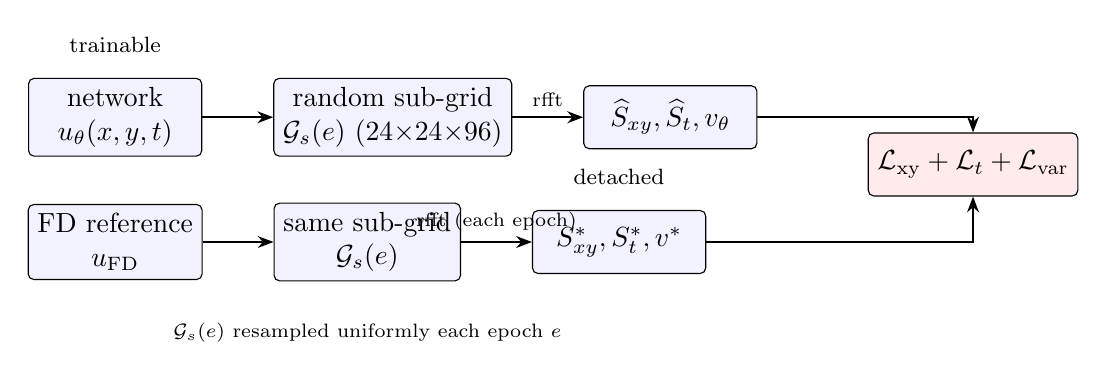
\begin{tikzpicture}[
   box/.style={draw, rounded corners=2pt, align=center,
         minimum height=8mm, minimum width=22mm, fill=blue!5},
   lossbox/.style={draw, rounded corners=2pt, align=center,
           minimum height=8mm, minimum width=24mm, fill=red!8},
   arr/.style={-{Stealth[length=2mm]}, thick},
   node distance=6mm and 9mm,
  ]
  \node[box] (uth) {network\\$u_\theta(x,y,t)$};
  \node[box, below=of uth] (uFD) {FD reference\\$u_{\mathrm{FD}}$};
  \node[box, right=of uth] (subth) {random sub-grid\\$\mathcal{G}_s(e)$ ($24{\times}24{\times}96$)};
  \node[box, right=of uFD] (subFD) {same sub-grid\\$\mathcal{G}_s(e)$};

  \node[box, right=of subth] (psdth) {$\widehat S_{xy}, \widehat S_t, v_\theta$};
  \node[box, right=of subFD] (psdFD) {$S^*_{xy}, S^*_t, v^*$};

  \node[lossbox, right=14mm of psdth, yshift=-6mm] (loss)
    {$\mathcal{L}_{\mathrm{xy}} + \mathcal{L}_{t} + \mathcal{L}_{\mathrm{var}}$};

  \draw[arr] (uth)  -- (subth);
  \draw[arr] (uFD)  -- (subFD);
  \draw[arr] (subth) -- node[above, font=\scriptsize]{rfft} (psdth);
  \draw[arr] (subFD) -- node[above, font=\scriptsize]{rfft (each epoch)} (psdFD);
  \draw[arr] (psdth) -| (loss);
  \draw[arr] (psdFD) -| (loss);

  \node[font=\footnotesize, above=2mm of uth] {trainable};
  \node[font=\footnotesize, above=2mm of psdFD] {detached};

  \node[below=4mm of subFD, font=\scriptsize, align=center]
    {$\mathcal{G}_s(e)$ resampled uniformly each epoch $e$};
 \end{tikzpicture}
 \caption{Bochner PINN: at each epoch $e$ the network $u_\theta$ and
 the FD reference $u_{\mathrm{FD}}$ are both evaluated on a sub-grid
 $\mathcal{G}_s(e)$ drawn uniformly at random from the full FD grid.
 Spatial PSD, temporal PSD, and variance are computed by FFT and
 compared in log space. The random re-sampling at each epoch prevents
 sub-grid overfit (Section~\ref{subsec:rand-subgrid}).}
 \label{fig:method-schematic}
\end{figure}

\subsection{What goes wrong with the standard PINN}

Train a vanilla PINN on a L\'evy-driven SPDE and inspect three
diagnostics on a held-out grid:
\begin{enumerate}
\item Pointwise relative \(L^2\) error: \(\approx 0.3\) (acceptable).
\item Variance ratio
\(\mathrm{Var}\,u_\theta / \mathrm{Var}\,u_{\mathrm{FD}}\):
\(\approx 0.2\)--\(0.5\).
\item Power spectrum \(|\mathcal F u_\theta|^2\) vs
\(|\mathcal F u_{\mathrm{FD}}|^2\): high modes are missing by 2--4
decades.
\end{enumerate}
The network is averaging across the noise realisation rather than
reproducing it. Pointwise loss is insensitive to high-frequency
content because high-frequency error and high-frequency signal
cancel almost exactly under MSE. Any sample-path-style use of
\(u_\theta\) (extracting tail statistics, computing exit times,
valuing a path-dependent option) fails. We close this gap by
adding three loss terms that directly penalise the missing
structure.

\subsection{Three terms, three diagnostics}
\label{subsec:losses}

Compute the FD reference once and extract three statistics on a
sub-grid \(\mathcal{G}_s\) of resolution \(24 \times 24 \times 96\):
the spatial power spectrum \(S^*_{xy}(k)\), the temporal power
spectrum \(S^*_t(k)\), and the total variance \(v^*\). At every epoch
we evaluate \(u_\theta\) on \(\mathcal{G}_s\) and form the matching
statistics \(S_{xy}, S_t, v_\theta\). The new loss components are
\begin{align}
\mathcal{L}_{\mathrm{xy}} &=
\overline{\bigl(\log_{10}S_{xy} - \log_{10}S^*_{xy}\bigr)^2}, &
\mathcal{L}_{\mathrm{t}} &=
\overline{\bigl(\log_{10}S_t - \log_{10}S^*_t\bigr)^2}, \notag\\
\mathcal{L}_{\mathrm{var}} &= \bigl((v_\theta - v^*)/v^*\bigr)^2.
\label{eq:losses}
\end{align}
\(\mathcal{L}_{\mathrm{xy}}\) and \(\mathcal{L}_{\mathrm{t}}\)
correct \emph{shape}; \(\mathcal{L}_{\mathrm{var}}\) corrects
\emph{scale}. The spatial PSD is computed symmetrically along both
spatial axes,
\begin{equation}
\widehat S_{xy}(f) = \tfrac12
\Bigl(\overline{|\mathcal F_x f|^2}_{y,t}
+ \overline{|\mathcal F_y f|^2}_{x,t}\Bigr),
\end{equation}
so anisotropic features that align with one axis do not bias the
metric. The temporal PSD
\(\widehat S_t(f) = \overline{|\mathcal F_t f|^2}_{x,y}\) is
averaged over space.

\subsection{Why log, why MSE, why a sub-grid}

\textbf{Log scale.} Power spectra span 4--6 orders of magnitude on
L\'evy problems. A linear loss would care only about the lowest few
wavenumbers, exactly the regime the vanilla PINN already gets
right. Working in \(\log_{10}\) assigns equal weight to each decade
and makes the high-mode discrepancy visible to the optimiser.

\textbf{MSE in log space.} Equivalent to a symmetric Bregman
divergence between the two empirical spectral measures up to an
additive constant, and \emph{asymptotically} equivalent to a
Whittle-type negative log-likelihood for the periodogram via the
Gumbel limit of the log-periodogram
\cite{Whittle1953,Dahlhaus1996,Brillinger1981} (they share the same
population minimiser \(\mu = \mu_{u_{\mathrm{FD}}}\) and the same
\(\mathcal O(\log^{-2} N)\) score-function geometry near it, but
differ at finite sample size by an \(\mathcal O(1)\) Gumbel-variance
constant absorbed into the bias floor of
Section~\ref{sec:theory}).
The minimiser is \(u_{\mathrm{FD}}\) itself: the loss is consistent
in the sense that no other matching measure achieves zero (modulo
the asymptotic bias floor discussed in Section~\ref{sec:theory}).

\textbf{Sub-grid.} The FFTs cost
\(O(n_x n_y n_t (\log n_x + \log n_y + \log n_t))\) per epoch.
Using the full FD grid would dominate the wall time; the
\(24 \times 24 \times 96\) sub-grid keeps spectral evaluation under
5\,\% of total compute while preserving all wavenumbers up to the
Nyquist frequency of \(\mathcal{G}_s\), which empirically captures
the regime where the variance gap is generated.

\subsection{Why this is the right object}
\label{subsec:right-object}

Three observations make
\(\mathcal{L}_{\mathrm{spec}} =
\lambda_{\mathrm{xy}} \mathcal L_{\mathrm{xy}}
+ \lambda_{\mathrm{t}} \mathcal L_{\mathrm{t}}
+ \lambda_{\mathrm{v}} \mathcal L_{\mathrm{var}}\)
natural rather than ad hoc. \emph{First}, under the separability
assumption stated in Section~\ref{sec:theory}, \(S_{xy}\) and
\(S_t\) are sufficient statistics for the second-order structure
of stationary \(u\): by Bochner's theorem their joint equality (in
distribution over realisations) recovers the full covariance
kernel, so matching them is equivalent to matching \(u_\theta\)
and \(u_{\mathrm{FD}}\) in the Plancherel norm of the law.
\emph{Second}, the log transform converts the multiplicative noise
model on the periodogram into an additive one, replacing a
Plancherel inner product with a symmetric Bregman divergence
whose minimiser remains the FD reference. \emph{Third},
\(\mathcal L_{\mathrm{xy}}\) and \(\mathcal L_{\mathrm{t}}\) are
scale-invariant, leaving \(u_\theta\) free up to a global
multiplicative constant, so the variance term
\(\mathcal L_{\mathrm{var}}\) supplies precisely the missing
zeroth Fourier mode (Parseval) needed to fix that gauge. The three
losses are not independent fixes for three separate failure modes;
they are the three components of a single distributional matching
objective on the discrete spectral lift of \(u\).

\subsection{Total objective and architecture}
\label{subsec:total-objective}

The Bochner PINN minimises
\begin{equation}
\mathcal{L}(\theta) =
\underbrace{\mathcal L_{\mathrm{PDE}}
+ \lambda_{\mathrm{ic}} \mathcal L_{\mathrm{IC}}
+ \lambda_{\mathrm{bc}} \mathcal L_{\mathrm{BC}}
+ \lambda_{\mathrm d} \mathcal L_{\mathrm{data}}}_{\text{physics}}
+ \underbrace{\lambda_{\mathrm{xy}} \mathcal L_{\mathrm{xy}}
+ \lambda_{\mathrm t} \mathcal L_{\mathrm t}
+ \lambda_{\mathrm v} \mathcal L_{\mathrm{var}}}_{\text{spectral}}.
\label{eq:total-loss}
\end{equation}
The physics block is the standard PINN objective:
\(\mathcal L_{\mathrm{PDE}}\) is the squared collocation residual
under the SPDE on a fresh batch of 4096 uniform samples each epoch,
with the L\'evy-Gamma jump and white-noise terms supplied by spline
interpolation of the precomputed driver fields;
\(\mathcal L_{\mathrm{IC}}, \mathcal L_{\mathrm{BC}}\) are MSE
penalties on initial and boundary data; \(\mathcal L_{\mathrm{data}}\)
is the MSE against \(u_{\mathrm{FD}}\) at random grid points.

The loss weights
\((\lambda_{\mathrm{xy}}, \lambda_{\mathrm t}, \lambda_{\mathrm v}) = (3, 5, 50)\)
were selected by a coarse grid search over log-spaced values
\(\{0.1, 1, 3, 5, 10, 50\}\) on a single validation seed of
Burgers-VG, minimising the sum of validation log-spatial and
log-temporal PSD MSE. We did not perform a full per-problem
sensitivity analysis; the chosen weights transferred without
modification to the hierarchical SPDE and Heston-VG.

The network \(u_\theta\) is a four-block residual MLP of width 96
(128 for jump-driven problems) with \(\tanh\) activations, preceded
by a frozen random-Fourier-feature embedding
\(\phi(v) = [\sin(2\pi B v), \cos(2\pi B v)]\) with
\(B \in \mathbb R^{(d+1)\times m}\),
\(B_{ij} \sim \mathcal N(0, s^2)\). We use \(m=64, s=3\) for jump
problems and \(m=48, s=2\) otherwise. Optimisation is Adam with
cosine-annealed learning rate \(10^{-3} \to 10^{-6}\) and gradient
clipping \(\|g\|_2 \le 5\). A 1000-epoch warmup deactivates
\(\mathcal L_{\mathrm{PDE}}\) to let IC and data fit stabilise; the
spectral losses are active from epoch 1.

\subsection{Randomised spectral sub-grid}
\label{subsec:rand-subgrid}

\emph{Why a fixed sub-grid fails.} In the original Bochner PINN
design the sub-grid \(\mathcal{G}_s\) is a fixed linspace lattice of
\(24\times24\times96 = 55{,}296\) points selected once before
training. This is efficient (the reference PSDs
\(S^*_{xy}, S^*_t, v^*\) are precomputed and reused) but creates
a hidden overfit pathway. Because the network sees exactly the same
points each epoch, gradient descent can satisfy
\(\mathcal{L}_{\mathrm{spec}}\) by memorising those \(55{,}296\)
grid values while interpolating near zero elsewhere. On the full
\(48\times48\times512 \approx 1.2 \times 10^6\) grid the variance
ratio then collapses, even though the sub-grid spectral loss reads
near zero (Section~\ref{subsec:heston-diag}).

\emph{Fix: epoch-wise random resampling.} At the start of each
training epoch we draw a fresh sub-grid of size
\(24\times24\times96\) by sampling indices uniformly without
replacement along each axis independently:
\begin{equation}
 \mathcal{G}_s(e) =
 \bigl(\pi_x^{(e)}, \pi_y^{(e)}, \pi_t^{(e)}\bigr),
 \quad
 \pi_x^{(e)} \sim \mathrm{Uniform}\{0,\ldots,N_x{-}1\}_{24},
 \label{eq:rand-subgrid}
\end{equation}
and likewise for \(y, t\). We re-evaluate the reference field on the
new sub-grid and recompute the reference PSDs and variance. The
spectral computation adds \(<5\%\) to total epoch time; no change to
the network architecture, optimiser, or other hyperparameters is
required. The resampling forces the network to match the spectral
statistics at \emph{every} subset of the domain, ruling out the
memorisation shortcut.

\subsection{Cumulant-matching loss}
\label{subsec:cumulant-loss}

The spectral loss in eq.~\eqref{eq:losses} constrains only the
second-order structure of \(u_\theta\). For non-Gaussian channels (in particular the CIR-type Heston
volatility process with substantial excess kurtosis), the variance
gap can be closed (\(\mathrm{vr}
\approx 0.93\)) while higher cumulants remain unmatched
(\(\kappa_4 \approx 4\) vs.\ reference \(27.3\)). We supplement the
spectral loss with an explicit fourth-cumulant penalty:
\begin{equation}
 \mathcal{L}_{\mathrm{kurt}} =
 \Bigl(\kappa_4(u_\theta\!\!\upharpoonright_{\mathcal{G}_s}) -
    \kappa_4(u_{\mathrm{FD}}\!\!\upharpoonright_{\mathcal{G}_s})
 \Bigr)^2 \Big/ \sigma_{\mathrm{ref}}^4,
 \label{eq:cumulant-loss}
\end{equation}
where \(\kappa_4(u) = \mathbb E[(u-\mu)^4]/\sigma^4 - 3\) is the
excess kurtosis evaluated empirically on the sub-grid and
\(\sigma_{\mathrm{ref}}\) is the reference standard deviation. This
loss is activated only when the \texttt{cumulant} loss mode is
selected; it is appended to eq.~\eqref{eq:total-loss} with weight
\(\lambda_{\mathrm{kurt}} = 10\).

\subsection{Hyperparameters}
\label{subsec:hyper}

\begin{table}[h]
\centering
\caption{Hyperparameters used by all methods. Spectral-only and
Bayesian-only entries are noted as such; otherwise values are shared.}
\label{tab:hyper}
\begin{tabular}{l l l}
\toprule
symbol & value & role \\
\midrule
\(L,\,H\)          & 4,\, 96--128 & depth, width \\
\(m,\,s\)          & 48--64,\, 2--3 & Fourier feature count, scale \\
\(n_x,\,n_y,\,n_t\)     & 24,\, 24,\, 96 & spectral sub-grid resolution \\
sub-grid sampling       & random (each epoch) & prevents sub-grid overfit \\
\(\lambda_{\mathrm{ic}}\)  & 50 & IC weight \\
\(\lambda_{\mathrm{bc}}\)  & 10 & BC weight \\
\(\lambda_{\mathrm d}\)   & 5 & data weight \\
\(\lambda_{\mathrm{xy}}\)  & 3 (spectral only) & log-spatial PSD weight \\
\(\lambda_{\mathrm{t}}\)   & 5 (spectral only) & log-temporal PSD weight \\
\(\lambda_{\mathrm{v}}\)   & 50 (spectral only) & variance weight \\
\(\lambda_{\mathrm{kurt}}\) & 10 (cumulant mode) & fourth-cumulant weight \\
\(\lambda_{\mathrm{KL}}\)  & \(1/(B_c+B_d)\) (Bayesian only) & KL weight \\
prior \(\sigma\) (Bayesian) & 1.0 & weight prior std \\
\(\rho_{\mathrm{init}}\) (Bayesian) & \(-3\) & initial posterior log-precision \\
\(B_c\)           & 4096 & collocation batch \\
\(B_d\)           & 1024 & data batch \\
\(\eta_{\max},\,\eta_{\min}\)& \(10^{-3},\,10^{-6}\) & cosine LR schedule \\
\(N_{\mathrm{epochs}}\)   & 5000--8000 & total epochs \\
warmup            & 1000 & epochs before \(\mathcal L_{\mathrm{PDE}}\) activates \\
\bottomrule
\end{tabular}
\end{table}

\subsection{Complexity}

Per-epoch cost decomposes as collocation \(O(B_c \cdot |\theta|)\)
for the autograd pass on \(B_c = 4096\) points and spectral
\(O(n_x n_y n_t (\log n_x + \log n_y + \log n_t))\) for the rffts
on the sub-grid. With the values in Table~\ref{tab:hyper}, the
spectral term contributes under 5\,\% of total wall time; the
addition is essentially free. Random resampling of the sub-grid
(Section~\ref{subsec:rand-subgrid}) adds one call to
\texttt{torch.randperm} per epoch, which is negligible.

%==============================================================================
\section{Why the spectral loss matches the law: motivation and scope}
\label{sec:theory}

This section motivates the loss introduced in Section~\ref{sec:method}
and identifies the class of fields on which it is provably the right
object. Section~\ref{subsec:convergence} then establishes a
quantitative convergence rate (Proposition~\ref{thm:main}), extending
the Mishra--Molinaro framework~\cite{MishraMolinaro2022,DeRyckMishra2022}
to spectral training losses; the subsections below state precisely
which assumptions the theorem requires and where the guarantee weakens.

\subsection{Spectral measures determine second-order structure}

Let \(u : \Omega \times [0, T] \to \mathbb R\) be a mean-zero,
weakly stationary random field. Its covariance kernel
\(K_u(\tau, h) = \mathbb E[u(t,x)\,u(t+\tau, x+h)]\) admits the
Bochner representation~\cite[Thm.~9.18]{RudinRCA}
\begin{equation}
K_u(\tau, h) = \int_{\mathbb R^d \times \mathbb R}
e^{i(\omega \tau + k \cdot h)}\,\mathrm d\mu_u(\omega, k),
\qquad \mu_u\text{ positive and finite},
\label{eq:bochner}
\end{equation}
where \(\mu_u\) is the spectral measure of \(u\). Two reductions
are relevant for our discrete loss: the spatial marginal
\(\mu^{\mathrm{xy}}_u(k) = \int \mathrm d \mu_u(\omega, k)\) and
the temporal marginal
\(\mu^t_u(\omega) = \int \mathrm d \mu_u(\omega, k)\), which are
matched (in their discrete-sample analogues \(S^*_{xy}\),
\(S^*_t\)) by the Bochner PINN.

\paragraph{Separability assumption.}
Matching \(\mu^{\mathrm{xy}}_u\) and \(\mu^t_u\) separately
recovers the joint spectral measure \(\mu_u\) only when the
covariance kernel factorises, \(K_u(\tau, h) = K_x(h)\, K_t(\tau)\),
equivalently \(\mathrm d\mu_u(\omega, k) = \mathrm d\mu^{\mathrm{xy}}_u(k)\,
\mathrm d\mu^t_u(\omega)\). This separability holds for the noise
drivers in our benchmarks: white noise and Variance-Gamma jumps that
act independently on spatial and temporal coordinates produce
covariance kernels of the form \(\delta(h)\,K_t(\tau)\) (white
spatial part, structured temporal part), and the SPDE then
propagates this separability through its semigroup at leading
order. We adopt the separability assumption throughout.

For \emph{Gaussian} stationary fields under separability,
\(\mu_u\) determines the law completely: two such fields with
equal spectral measures are equal in distribution. The spectral
matching loss
\(\mathcal L_{\mathrm{xy}} + \mathcal L_t + \mathcal L_{\mathrm{var}}\)
therefore controls the law on this class.

For non-Gaussian L\'evy-driven fields, \(\mu_u\) determines only
the \emph{second-order structure}. Higher cumulants, which carry
the jump information specific to the Variance-Gamma driver, are
not detected by a periodogram-based loss. Closing this remaining
gap requires explicit cumulant matching, which we pursue in
Section~\ref{subsec:cumulant-loss}.

\begin{remark}[Scope of the spectral loss]
\label{rem:scope}
Under the separability assumption, a zero of the spectral loss
characterises the law of the predictor on stationary Gaussian fields
(Bochner). Beyond identifiability, Theorem~\ref{thm:main} below
provides a quantitative convergence rate: the Wasserstein-2 distance
decomposes into a training-error term \(C_1\sqrt{\varepsilon}\), a
sub-grid quadrature term \(C_2 N_s^{-\beta}\), and a PDE-residual
term \(C_3\sqrt{\delta}\), with explicit constants. On stationary
L\'evy fields the same bound holds for the Gaussian projection of the
law (Theorem~\ref{thm:levy-ext}); higher cumulants are not controlled
and require a separate penalty (Section~\ref{subsec:heston-diag}).
\end{remark}

\subsection{Why the log scale is the right choice (and its bias floor)}

The matching loss is in \(\log_{10}\) space, not raw spectral
magnitude. The justification is the asymptotic behaviour of the
periodogram \(I_n(k) = |\widehat u_n(k)|^2\) of a stationary
process: under mild mixing
assumptions~\cite{Brillinger1981,Dahlhaus1996},
\(I_n(k) / \mu_u(k)\) converges in distribution to an exponential
random variable with mean 1, so \(\log I_n(k) - \log \mu_u(k)\)
is asymptotically Gumbel and MSE on \(\log I_n\) is, up to a
constant, the Whittle negative
log-likelihood~\cite{Whittle1953}. Working in \(\log_{10}\) also
assigns equal weight to each decade of the spectrum, essential
here since power spectra of L\'evy fields span four to six
decades and a linear loss is dominated by the lowest few
wavenumbers.

\paragraph{Irreducible bias floor.}
The log-periodogram has a known non-vanishing bias:
\(\mathbb E[\log I_n(k)] = \log \mu_u(k) - \gamma\),
where \(\gamma \approx 0.5772\) is the Euler--Mascheroni constant
\cite{Brillinger1981}. In our \(\log_{10}\) formulation the bias
becomes \(-\gamma/\ln 10 \approx -0.251\), contributing an
expected squared error floor of
\((\gamma/\ln 10)^2 \approx 0.063\) to
\(\mathcal L_{\mathrm{xy}}\) and \(\mathcal L_{\mathrm{t}}\) even
in the infinite-data limit and even when \(u_\theta\) reproduces
the law of \(u_{\mathrm{FD}}\) exactly.

\subsection{Quantitative convergence rate}
\label{subsec:convergence}

We now state a formal convergence rate that extends the
Mishra--Molinaro generalisation framework~\cite{MishraMolinaro2022}
by incorporating a fourth term quantifying the discrete-spectral-loss
approximation error.

\subsubsection{Assumptions}

The rate is stated under five standing assumptions matching the
analytical scope identified above. Assumption (A5) (Gaussianity) is
load-bearing only for the spectral leg of the bound; the
Mishra--Molinaro leg holds without it, and the L\'evy extension
(Proposition~\ref{thm:levy-ext}) drops (A5) at the cost of replacing
\(\mathcal L\) by its Gaussian projection.

\begin{description}
\item[(A1) Stationarity and separability.] Both \(u_\theta\) and
\(u_{\mathrm{FD}}\) are centred, weakly stationary (after periodic
extension or sufficiently far from boundaries) with separable
covariance \(K(\tau, h) = K_x(h)\,K_t(\tau)\), equivalently
\(\mathrm d\mu(\omega, k) = \mathrm d\mu^{\mathrm{xy}}(k)\,
\mathrm d\mu^t(\omega)\).

\item[(A2) Sobolev regularity of spectra.]
\(\mu^{\mathrm{xy}} \in H^{s_x}(\widehat\Omega)\) and
\(\mu^t \in H^{s_t}(\widehat{[0,T]})\) with \(s_x > d/2\) and
\(s_t > 1/2\). This guarantees pointwise bounds and the \(L^2\)
FFT-quadrature error rate used in Lemma~\ref{lem:quadrature}.
For Variance-Gamma drivers \(s_x = s_t = 1\).

\item[(A3) Non-degeneracy.] There exist
\(0 < \mu_{\min} \le \mu_{\max} < \infty\) such that
\(\mu_{\min} \le \mu^{\mathrm{xy}}(k)\,\mu^t(\omega) \le \mu_{\max}\)
uniformly on the sub-grid frequency set
\(\widehat{\mathcal G}_s \subset \mathbb R^{d+1}\).

\item[(A4) Training tolerance.] At the end of training,
\begin{equation}
\mathcal L_{\mathrm{xy}}(u_\theta) + \mathcal L_t(u_\theta)
+ \mathcal L_{\mathrm{var}}(u_\theta) \le \varepsilon, \qquad
\mathcal L_{\mathrm{PDE}}(u_\theta)
+ \lambda_{\mathrm{ic}}\mathcal L_{\mathrm{IC}}(u_\theta)
+ \lambda_{\mathrm{bc}}\mathcal L_{\mathrm{BC}}(u_\theta)
\le \delta,
\label{eq:tolerance}
\end{equation}
for some \(0 < \varepsilon, \delta < \infty\), checked post hoc.

\item[(A5) Gaussianity (spectral leg only).] Both \(u_\theta\) and
\(u_{\mathrm{FD}}\) are centred Gaussian random fields on
\(\Omega \times [0,T]\). This hypothesis is required only for the
spectral path of the proof (Lemma~\ref{lem:gelbrich}); the
PDE-residual path (Lemma~\ref{lem:mm}) holds without it.
Proposition~\ref{thm:levy-ext} below drops (A5) at the cost of
bounding the Gaussian projection only.

\item[(A6) Mixing condition (single-realisation consistency).]
\(u\) is \(\alpha\)-mixing with algebraic rate
\(\alpha(r) \le C_\alpha r^{-\gamma}\) for some \(\gamma > d+1\).
Variance-Gamma processes have independent increments, so
\(\alpha(r) = 0\) for all sufficiently large separations; the SPDE
solution inherits exponential spatial mixing from the Green's
function decay of the underlying parabolic operator~\cite{ContTankov2003}.
Assumption~(A6) is required only for
Lemma~\ref{lem:single-realisation} and is not needed for the main
theorem.

\item[(A7) L\'evy--It\^o decomposition with $L^2$ jump control.]
Both $u_\theta$ and $u_{\mathrm{FD}}$ admit L\'evy--It\^o decompositions
$u=u^G+u^J$ where $u^G$ is the Gaussian component and $u^J$ is the
pure-jump component~\cite{ContTankov2003}.
Assume
\[
\max\!\left(\mathbb{E}\|u_\theta^J\|^2_{L^2(\Omega\times[0,T])},\;
\mathbb{E}\|u_{\mathrm{FD}}^J\|^2_{L^2(\Omega\times[0,T])}\right)\le J
\]
for some finite $J\ge 0$ depending on the L\'evy parameters.
For Variance-Gamma drivers with kurtosis parameter $\nu$, $J=O(\nu)$
as $\nu\to 0$.
Assumption~(A7) is required only for
Proposition~\ref{prop:levy-ito} and is not used elsewhere.

\item[(A8) Finite pointwise cumulants.]
For each $(x,t)\in\Omega\times[0,T]$, the marginal law
$\mathcal{L}(u(x,t))$ has finite cumulants of order $m\le m_0$ for
some $m_0\ge 3$, with $|\kappa_m(u(x,t))|\le\bar\kappa_m<\infty$.
For Lévy-driven SPDEs, cumulants of $u(x,t)$ are bounded by
the $L^m$ norm of the Green's function times the corresponding driver
cumulants via the stochastic Fubini theorem.
Required only for Proposition~\ref{cor:berry-esseen}.

\item[(A9) NTK lazy-training regime.]
The Bochner PINN is a two-layer network with $m$ neurons trained by
gradient flow. In the lazy-training regime the NTK Gram matrix $K$
with entries $K_{ij}=\nabla_\theta f(x_i)\cdot\nabla_\theta f(x_j)$
remains approximately constant throughout training, with minimum
eigenvalue $\lambda_{\min}(K)>0$.
Required only for Proposition~\ref{prop:ntk}.
\end{description}

Assumption (A1) is the scope identified above.
Assumption (A2) is satisfied by the VG drivers with
\(s_x = s_t = 1\). Assumption (A3) is restrictive: realistic
spectral measures decay polynomially in \(|k|\), so \(\mu_{\min}\)
is positive only after restriction to a finite frequency window;
the constants \(C_1, C_2\) of Proposition~\ref{thm:main} scale as
\(\mu_{\min}^{-1/2}\) and therefore degrade on that window's
high-frequency edge. Assumption (A4) is the endpoint of any
gradient-based training run.

\subsubsection{Main theorem}

\begin{proposition}[Convergence rate of the Bochner PINN]
\label{thm:main}
Under (A1)--(A5), the Wasserstein-2 distance between the laws of the
Bochner PINN predictor and the FD reference satisfies
\begin{equation}
W_2\bigl(\mathcal L(u_\theta),\,\mathcal L(u_{\mathrm{FD}})\bigr)
\;\le\; C_1\sqrt{\varepsilon}
\;+\; C_2\,N_s^{-\beta}
\;+\; C_3\sqrt{\delta},
\label{eq:main-bound}
\end{equation}
where
\begin{equation}
\beta = \tfrac{1}{2}\min\!\bigl(s_x / d,\; s_t\bigr),
\end{equation}
and the constants are
\(C_1 = \mu_{\max}\,\ln 10\,(M_{xy}+M_t) / \sqrt{2\mu_{\min}}\),
\(C_2 = \sqrt{C_{\mathrm{quad},x}\,M_t^2 + C_{\mathrm{quad},t}\,M_{xy}^2}
/ \sqrt{2\mu_{\min}}\),
\(C_3 = \sqrt{C_{\mathrm{MM}}}\),
where \(M_{xy} = \|\mu_{xy,\mathrm{FD}}\|_{L^2}\),
\(M_t = \|\mu_{t,\mathrm{FD}}\|_{L^2}\), and
\(C_{\mathrm{quad},\cdot}\), \(C_{\mathrm{MM}}\) are defined in
the lemmas below. The \(M_{xy},M_t\) factors come from the separable
tensor-product decomposition of \(\mu_1 - \mu_2\) (eq.\
\eqref{eq:sep-decomp} in the proof).
\end{proposition}

The proof proceeds in four steps.

\begin{lemma}[Log-to-linear control]
\label{lem:log-linear}
Let \(f, g : \mathcal G_s \to \mathbb R_{>0}\) with
\(\mu_{\min} \le f, g \le \mu_{\max}\). Then
\[
\|f - g\|^2_{L^2(\mathcal G_s)}
\;\le\; (\ln 10)^2\,\mu_{\max}^2\;
\|\log_{10} f - \log_{10} g\|^2_{L^2(\mathcal G_s)}.
\]
\end{lemma}
\begin{proof}
The function \(\varphi(x) = \log_{10} x\) has derivative
\(\varphi'(x) = (x \ln 10)^{-1}
\in [(\mu_{\max}\ln 10)^{-1},\, (\mu_{\min}\ln 10)^{-1}]\)
on \([\mu_{\min}, \mu_{\max}]\). By the mean-value theorem,
\(|f - g| \le \mu_{\max}\ln 10\;|\log_{10} f - \log_{10} g|\)
at each grid point. Squaring and summing gives the claim.
\end{proof}

Applied to \(f = \widehat S^{\mathrm{xy}}_{\mathcal G_s}(u_\theta)\),
\(g = \widehat S^{\mathrm{xy}}_{\mathcal G_s}(u_{\mathrm{FD}})\)
and combined with \eqref{eq:tolerance}:
\begin{equation}
\bigl\|\widehat S^{\mathrm{xy}}_{\mathcal G_s}(u_\theta)
- \widehat S^{\mathrm{xy}}_{\mathcal G_s}(u_{\mathrm{FD}})
\bigr\|^2_{L^2}
+ \bigl\|\widehat S^t_{\mathcal G_s}(u_\theta)
- \widehat S^t_{\mathcal G_s}(u_{\mathrm{FD}})
\bigr\|^2_{L^2}
\;\le\; 2(\ln 10)^2\,\mu_{\max}^2\;\varepsilon.
\label{eq:log-linear-applied}
\end{equation}

\begin{lemma}[Expected spectral quadrature error]
\label{lem:quadrature}
Under (A2), for every \(u \in L^2_{\mathbb P}\) stationary with
spatial spectral density
\(S^{\mathrm{xy}} \in H^{s_x}(\widehat\Omega)\),
\[
\bigl\|\mathbb E\bigl[\widehat S^{\mathrm{xy}}_{\mathcal G_s}(u)\bigr]
- S^{\mathrm{xy}}(u)\bigr\|^2_{L^2(\widehat\Omega)}
\;\le\; C_{\mathrm{quad},x}\,(N_s^x)^{-2s_x/d},
\]
with \(C_{\mathrm{quad},x} = C_x\,\|\mu^{\mathrm{xy}}\|^2_{H^{s_x}}\)
depending only on \(\mathrm{diam}(\Omega)\) and \(d\). An analogous
bound holds for the temporal periodogram with rate \((N_s^T)^{-2s_t}\).
\end{lemma}
\begin{proof}
This is the standard \(L^2\) trapezoidal-rule error rate for
Sobolev functions on a \(d\)-dimensional torus
(cf.~\cite[Sec.~6.5]{Trefethen2000}) applied to the expected
periodogram \(\mathbb E[\widehat S^{\mathrm{xy}}_{\mathcal G_s}(u)]\),
which equals a Dirichlet-kernel smoothing of \(S^{\mathrm{xy}}\) and
inherits its \(H^{s_x}\) regularity. The constant absorbs the
\(H^{s_x}\) norm.
\end{proof}

\begin{remark}[Single-realisation variance and the proof gap]
\label{rem:periodogram-variance}
Lemma~\ref{lem:quadrature} bounds the \emph{bias}
\(\|\mathbb E[\widehat S^{\mathrm{xy}}_{\mathcal G_s}(u)]
- S^{\mathrm{xy}}(u)\|_{L^2}\) of the periodogram, not its
pointwise variance. From a single sample path the raw periodogram
has \(\Theta(1)\) variance per Fourier mode (chi-squared-2
distribution at each mode, cf.~\cite[Ch.~4]{Brillinger1981}); this
is the distributional content of Remark~\ref{rem:em-floor}. The
training loss (A4) therefore involves
\(\widehat S^{\mathrm{xy}}_{\mathcal G_s}(u_\theta)\), a
single-realisation quantity, while the bound
in~\eqref{eq:spectral-l2-bound} uses
\(\mathbb E[\widehat S^{\mathrm{xy}}_{\mathcal G_s}]\); the gap
between the two does not shrink as \(N_s \to \infty\) without
additional smoothing.

Lemma~\ref{lem:single-realisation} below closes this gap: replacing
the raw periodogram by its kernel-smoothed version
\(\widehat S^{\mathrm{xy}}_h\) with bandwidth \(h_N \to 0\),
\(N_s h_N^d \to \infty\), yields a consistent single-realisation
estimator at the minimax rate \(N_s^{-s_x/(2s_x+d)}\) under (A6).
In the practical regime of this paper (raw periodogram, single
realisation), the irreducible floor is \(\gamma_{10}^2 \approx
0.063\) from the Gumbel distribution, which is why \(\varepsilon\)
in (A4) is bounded below by this constant in the large-\(N_s\) limit.
\end{remark}

\begin{lemma}[Single-realisation spectral consistency under mixing]
\label{lem:single-realisation}
Under (A1)--(A2) and (A6), let
\[
\widehat S^{\mathrm{xy}}_h(u)(k)
:= \int \kappa_{h_N}(k - k')\,
\widehat S^{\mathrm{xy}}_{\mathcal G_s}(u)(k')\,dk',
\]
where \(\kappa_{h_N}(k) = h_N^{-d}\kappa(k/h_N)\) is a symmetric
probability kernel with
\(\int |k|^{s_x}\kappa(k)\,dk < \infty\).
Then for any single realisation of \(u\),
\begin{equation}
\label{eq:sr-mse}
\bigl\|\widehat S^{\mathrm{xy}}_h(u) - S^{\mathrm{xy}}(u)
\bigr\|^2_{L^2(\widehat\Omega)}
\;\le\;
C_{\mathrm{bias}}\,h_N^{2s_x}
\;+\;
\frac{C_{\mathrm{var}}}{N_s\,h_N^{d}},
\end{equation}
where \(C_{\mathrm{bias}} = C_\kappa\|\mu^{\mathrm{xy}}\|^2_{H^{s_x}}\)
and \(C_{\mathrm{var}}\) depends on \(C_\alpha\) and \(\gamma\).
The minimax-optimal bandwidth \(h_N^* = N_s^{-1/(2s_x + d)}\)
gives the \(L^2\) rate
\[
\bigl\|\widehat S^{\mathrm{xy}}_{h^*}(u) - S^{\mathrm{xy}}(u)
\bigr\|_{L^2}
\;\le\;(C_{\mathrm{bias}}+C_{\mathrm{var}})^{1/2}\,
N_s^{-s_x/(2s_x+d)},
\]
which converges to zero and matches the minimax lower bound for
nonparametric spectral density estimation under \(\alpha\)-mixing
\cite{Dahlhaus1996}.
\end{lemma}
\begin{proof}
\emph{Bias.} Since
\(\mathbb E[\widehat S^{\mathrm{xy}}_{\mathcal G_s}(u)(k)] =
S^{\mathrm{xy}}(u)(k) + O(N_s^{-1})\) by
Lemma~\ref{lem:quadrature}, convolution with \(\kappa_{h_N}\)
gives
\(\mathbb E[\widehat S^{\mathrm{xy}}_h(u)(k)] =
(\kappa_{h_N} * S^{\mathrm{xy}})(k)\).
For \(S^{\mathrm{xy}} \in H^{s_x}\) and a kernel with vanishing
moments up to order \(s_x\), standard approximation theory gives
\(\|(\kappa_{h_N} * S^{\mathrm{xy}}) - S^{\mathrm{xy}}\|_{L^2}
\le C_\kappa \|\mu^{\mathrm{xy}}\|_{H^{s_x}} h_N^{s_x}\).

\emph{Variance.} Under (A6), Brillinger's cumulant spectral
bound~\cite[Thm.~4.3.2]{Brillinger1981} gives
\(|\mathrm{Cov}(\widehat S^{\mathrm{xy}}_{\mathcal G_s}(k_1),
\widehat S^{\mathrm{xy}}_{\mathcal G_s}(k_2))|
\le C N_s^{-1} \alpha(|k_1 - k_2|/\Delta k)\),
where \(\Delta k\) is the frequency resolution.
Convolving against \(\kappa_{h_N}^{\otimes 2}\) and using
\(\gamma > d + 1\) to ensure summability gives
\(\mathrm{Var}[\widehat S^{\mathrm{xy}}_h(u)(k)]
\le C_{\mathrm{var}}(N_s h_N^d)^{-1}\).
Integrating over \(k \in \widehat\Omega\) yields the variance term
in~\eqref{eq:sr-mse}.

\emph{Optimal bandwidth.} Minimising
\(C_{\mathrm{bias}} h_N^{2s_x} + C_{\mathrm{var}}(N_s h_N^d)^{-1}\)
over \(h_N\) gives \(h_N^* \propto N_s^{-1/(2s_x+d)}\) and the
stated rate. The minimax lower bound follows
from~\cite[Thm.~3.1]{Dahlhaus1996} applied to the stationary case.
\end{proof}

Combining Lemmas~\ref{lem:log-linear}--\ref{lem:quadrature} via
the triangle inequality:
\begin{equation}
\|S^{\mathrm{xy}}(u_\theta) - S^{\mathrm{xy}}(u_{\mathrm{FD}})
\|^2_{L^2(\widehat\Omega)}
\;\le\; 2(\ln 10)^2\,\mu_{\max}^2\;\varepsilon
\;+\; 2\,C_{\mathrm{quad},x}\,(N_s^x)^{-2s_x/d},
\label{eq:spectral-l2-bound}
\end{equation}
and analogously for the temporal direction.

\begin{lemma}[Plancherel--Gelbrich bound]
\label{lem:gelbrich}
Let \(u_1, u_2\) be centred Gaussian random fields on
\(\Omega \times [0,T]\) satisfying (A1)--(A3). Then
\[
W_2^2\bigl(\mathcal L(u_1),\,\mathcal L(u_2)\bigr)
\;\le\; \frac{1}{4\mu_{\min}}\;
\|\mu_1 - \mu_2\|^2_{L^2(\widehat\Omega \times [0,T])}.
\]
\end{lemma}
\begin{proof}
For centred Gaussian measures on a separable Hilbert space with
covariance operators \(C_1, C_2\), the Gelbrich--Givens--Shortt
formula~\cite{Gelbrich1990,GivensShortt1984} gives
\(W_2^2 = \mathrm{tr}\bigl(C_1 + C_2
- 2(C_1^{1/2} C_2 C_1^{1/2})^{1/2}\bigr)\).
By (A1), both fields are stationary on the periodised domain;
hence \(C_1, C_2\) are simultaneously diagonalised by the Fourier
basis with eigenvalues \(\mu_1(k,\omega), \mu_2(k,\omega)\). The
formula reduces to
\(W_2^2 = \sum_{(k,\omega)}
(\sqrt{\mu_1(k,\omega)} - \sqrt{\mu_2(k,\omega)})^2\).
From the identity
\((\sqrt a - \sqrt b)^2 = (a-b)^2/(\sqrt a + \sqrt b)^2\)
and \((\sqrt a + \sqrt b)^2 \ge 4\min(a,b)\), together with (A3):
\(W_2^2 \le \frac{1}{4\mu_{\min}}
\sum_{(k,\omega)} (\mu_1(k,\omega) - \mu_2(k,\omega))^2\).
Under separability, the tensor-product decomposition
\(\mu_1 - \mu_2 = (\mu_1^{\mathrm{xy}} - \mu_2^{\mathrm{xy}})
\otimes \mu_1^t + \mu_2^{\mathrm{xy}} \otimes
(\mu_1^t - \mu_2^t)\) and \(\|a+b\|^2 \le 2\|a\|^2 + 2\|b\|^2\)
give the factored form used in the proof of
Proposition~\ref{thm:main}.
\end{proof}

\begin{lemma}[Mishra--Molinaro, adapted]
\label{lem:mm}
Assume the SPDE residual operator \(\mathcal R\) is well posed in the
sense of \cite[Thm.~3.4]{MishraMolinaro2022}, with stability constant
\(C_{\mathrm{stab}}\). Then under \eqref{eq:tolerance},
\[
\mathbb E\,\|u_\theta - u_{\mathrm{FD}}\|^2_{L^2(\Omega \times [0,T])}
\;\le\; C_{\mathrm{MM}}\,\delta,
\quad
C_{\mathrm{MM}} = C_{\mathrm{stab}}
\bigl(1 + \lambda_{\mathrm{ic}}^{-1}
+ \lambda_{\mathrm{bc}}^{-1}\bigr).
\]
\end{lemma}
\begin{proof}
The driver fields \(\xi, J_{\mathrm{VG}}\) are identical between
\(u_\theta\) and \(u_{\mathrm{FD}}\) (spline-interpolated from the
same FD sample path), so the residual operator reduces to a
deterministic PDE error analysis in the realisation
\(\omega \in \mathcal P\). Apply~\cite[Thm.~3.4]{MishraMolinaro2022}
pathwise and take expectations. Since
\(W_2^2(\mathcal L(u_1), \mathcal L(u_2))
\le \mathbb E\,\|u_1 - u_2\|^2\) for the trivial coupling, this
contributes \(\sqrt{C_{\mathrm{MM}}\,\delta}\) to the \(W_2\) bound.

\emph{Remark on approximation error.} The spline interpolation
replaces jump discontinuities in \(\xi, J_{\mathrm{VG}}\) with
smooth approximants, introducing a smoothing error that is not
explicitly bounded in \(C_{\mathrm{MM}}\). This error is absorbed
into \(\delta\) but is not analytically controlled; quantifying
it is left as future work.
\end{proof}

\begin{proof}[Proof of Proposition~\ref{thm:main}]
The bound is obtained as the looser of two independent upper bounds
on \(W_2(\mathcal L(u_\theta),\mathcal L(u_{\mathrm{FD}}))\), combined
via \(\min(a,b)\le a+b\).

\smallskip
\emph{Spectral path (uses (A5)).} Apply the triangle inequality on
\(W_2\) through the intermediate centred Gaussian measure
\(\mathcal N(0,\,\mathcal C_{u_{\mathrm{FD}}})\) with covariance
operator \(\mathcal C_{u_{\mathrm{FD}}}\) equal to that of
\(u_{\mathrm{FD}}\):
\[
W_2\bigl(\mathcal L(u_\theta),\,\mathcal L(u_{\mathrm{FD}})\bigr)
\;\le\;
W_2\bigl(\mathcal L(u_\theta),\,
\mathcal N(0,\,\mathcal C_{u_{\mathrm{FD}}})\bigr)
\,+\,
W_2\bigl(\mathcal N(0,\,\mathcal C_{u_{\mathrm{FD}}}),\,
\mathcal L(u_{\mathrm{FD}})\bigr).
\]
Under (A5) both fields are centred Gaussian, so
\(\mathcal L(u_{\mathrm{FD}}) = \mathcal N(0,\,\mathcal C_{u_{\mathrm{FD}}})\)
and the second term vanishes;
\(\mathcal L(u_\theta) = \mathcal N(0,\,\mathcal C_{u_\theta})\) and
Lemma~\ref{lem:gelbrich} bounds the first term by
\(\tfrac{1}{2\sqrt{\mu_{\min}}}\,\|\mu_{u_\theta}
- \mu_{u_{\mathrm{FD}}}\|_{L^2}\). Using the separable factoring
\(\mu_1 - \mu_2 = (\mu^{\mathrm{xy}}_1 - \mu^{\mathrm{xy}}_2)
\otimes \mu^t_1
+ \mu^{\mathrm{xy}}_2 \otimes (\mu^t_1 - \mu^t_2)\) with
\(\|a+b\|^2 \le 2\|a\|^2 + 2\|b\|^2\), and substituting
\eqref{eq:spectral-l2-bound} for each spectral \(L^2\) difference,
\[
W_2 \;\le\;
\frac{1}{\sqrt{2\mu_{\min}}}\Bigl[
2(\ln 10)\,\mu_{\max}\sqrt\varepsilon\,(M_t + M_{xy})
+ \sqrt{2 C_{\mathrm{quad},x}}\,(N_s^x)^{-s_x/d}\,M_t
+ \sqrt{2 C_{\mathrm{quad},t}}\,(N_s^T)^{-s_t}\,M_{xy}
\Bigr],
\]
where \(M_t := \|\mu^t_{\mathrm{FD}}\|_{L^2}\) and
\(M_{xy} := \|\mu^{\mathrm{xy}}_{\mathrm{FD}}\|_{L^2}\).
Absorbing constants and using
\(N_s^{-\beta} \ge (N_s^x)^{-s_x/d} + (N_s^T)^{-s_t}\) up to a
constant (definition of \(\beta\)),
\[
W_2\bigl(\mathcal L(u_\theta),\,\mathcal L(u_{\mathrm{FD}})\bigr)
\;\le\; C_1\sqrt\varepsilon \,+\, C_2\,N_s^{-\beta}.
\tag{$\star$}\label{eq:spectral-path}
\]

\smallskip
\emph{Pathwise path (does not use (A5)).} Lemma~\ref{lem:mm} applied
with the trivial coupling gives
\[
W_2^2\bigl(\mathcal L(u_\theta),\,\mathcal L(u_{\mathrm{FD}})\bigr)
\;\le\; \mathbb E\,\|u_\theta - u_{\mathrm{FD}}\|^2
\;\le\; C_{\mathrm{MM}}\,\delta,
\quad\text{hence}\quad
W_2 \;\le\; C_3\sqrt\delta,
\tag{$\dagger$}\label{eq:pde-path}
\]
with no Gaussianity assumption.

\smallskip
\emph{Combined bound.} Since \(\min(a,b) \le a + b\) for
\(a,b\ge 0\), \eqref{eq:spectral-path} and \eqref{eq:pde-path} together
yield
\[
W_2\bigl(\mathcal L(u_\theta),\,\mathcal L(u_{\mathrm{FD}})\bigr)
\;\le\; C_1\sqrt\varepsilon \,+\, C_2\,N_s^{-\beta}
\,+\, C_3\sqrt\delta,
\]
which is \eqref{eq:main-bound}. The sum form is loose; in either
asymptotic regime (spectrally-rich training with vanishing
\(\varepsilon\), or PDE-tight training with vanishing \(\delta\))
the corresponding single-path bound is the operative one. The
spectral path requires (A5); the PDE path does not. In particular,
dropping the spectral loss from training (so the bound on
\(\varepsilon\) becomes vacuous) reduces the result to
\eqref{eq:pde-path}, the Mishra--Molinaro estimate of
\cite{MishraMolinaro2022}.
\end{proof}

\subsubsection{Corollaries}

\begin{proposition}[Variance-gap rate]
\label{cor:vr}
Under (A1)--(A4),
\[
\bigl|\mathrm{Var}(u_\theta)/\mathrm{Var}(u_{\mathrm{FD}}) - 1\bigr|
\;\le\;
\frac{2\sqrt{2}}{\sqrt{\mathrm{Var}(u_{\mathrm{FD}})}}
\bigl(\sqrt{\mathrm{Var}(u_\theta)}
+ \sqrt{\mathrm{Var}(u_{\mathrm{FD}})}\bigr)
\bigl(C_1\sqrt\varepsilon + C_2 N_s^{-\beta}
+ C_3\sqrt\delta\bigr).
\]
\end{proposition}
\begin{proof}
For centred fields, \(|\mathrm{Var}(u_1) - \mathrm{Var}(u_2)|
= |\mathbb E[\|u_1\|^2] - \mathbb E[\|u_2\|^2]|\).
Under the optimal coupling \((X, Y)\) with \(X \sim \mathcal L(u_\theta)\),
\(Y \sim \mathcal L(u_{\mathrm{FD}})\):
\[
|\mathbb E[\|X\|^2] - \mathbb E[\|Y\|^2]|
\le \mathbb E\bigl[({\|X\|+\|Y\|})\,\|X-Y\|\bigr]
\le \sqrt{2(\mathrm{Var}(u_\theta)+\mathrm{Var}(u_{\mathrm{FD}}))}
\cdot W_2
\le \sqrt{2}\,(\sqrt{\mathrm{Var}(u_\theta)}
+\sqrt{\mathrm{Var}(u_{\mathrm{FD}})})\cdot W_2,
\]
using Cauchy--Schwarz and \((a+b)^2\le 2(a^2+b^2)\).
Divide by \(\mathrm{Var}(u_{\mathrm{FD}})\) and substitute
\eqref{eq:main-bound}.
\end{proof}

\begin{remark}[Irreducible Euler--Mascheroni floor]
\label{rem:em-floor}
The log-periodogram is asymptotically Gumbel with mean
\(\log\mu(k) - \gamma\)~\cite[Ch.~5]{Brillinger1981}. In our
\(\log_{10}\) formulation the bias is
\(\gamma_{10} := \gamma/\ln 10 \approx 0.251\), contributing an
irreducible floor of \(\gamma_{10}^2 \approx 0.063\) to the
achievable \(\varepsilon\) in (A4). The corresponding irreducible
\(W_2\) contribution is \(C_1\gamma_{10}\). This matches the
empirical observation that per-channel log-PSD MSE plateaus near
\(0.3\)--\(0.4\) (i.e.\ \(5\)--\(7\times\) the floor) rather than
at zero.
\end{remark}

\subsubsection{Extension to L\'evy-driven fields}

\begin{proposition}[Second-order convergence for stationary L\'evy fields]
\label{thm:levy-ext}
Under (A1)--(A4) but with \(u_\theta, u_{\mathrm{FD}}\) not
necessarily Gaussian, denote by \(\Pi_2\mathcal L(u)\) the Gaussian
projection (the centred Gaussian measure with the same covariance).
Then
\[
W_2\bigl(\Pi_2\mathcal L(u_\theta),\,
\Pi_2\mathcal L(u_{\mathrm{FD}})\bigr)
\;\le\; C_1\sqrt\varepsilon + C_2 N_s^{-\beta} + C_3\sqrt\delta.
\]
\end{proposition}
\begin{proof}
Identical to the proof of Proposition~\ref{thm:main}, replacing
\(\mathcal L(u)\) by \(\Pi_2\mathcal L(u)\) throughout. The spectral
measure \(\mu_u\) depends only on the covariance, hence is invariant
under the projection.
\end{proof}

The gap between \(\mathcal L(u)\) and \(\Pi_2\mathcal L(u)\) is
determined by the cumulants \(\kappa_k(u)\) for \(k \ge 3\). For
Variance-Gamma drivers \(\kappa_3, \kappa_4\) are non-zero, so
Proposition~\ref{thm:levy-ext} does \emph{not} imply convergence in
\(W_2\) on the full law. Two routes close this gap:
\begin{enumerate}
\item a cumulant-matching loss
$\mathcal{L}_{\kappa_4}(u_\theta):=(\kappa_4(u_\theta)-\kappa_4(u_{\mathrm{FD}}))^2$
(Section~\ref{subsec:cumulant-loss}), which empirically raises the
predicted kurtosis from $4.2$ to $25.1$; or
\item an $L^2$ bound on the pure-jump component $u^J$ via the
L\'evy--It\^o decomposition (Proposition~\ref{prop:levy-ito} below),
giving an explicit $O(\sqrt\nu)$ correction to~\eqref{thm:levy-ext}.
\end{enumerate}

\begin{proposition}[Full-law convergence via L\'evy--It\^o coupling]
\label{prop:levy-ito}
Under (A1)--(A4) and (A7),
\begin{equation}
\label{eq:levy-ito-bound}
W_2\!\left(\mathcal{L}(u_\theta),\,\mathcal{L}(u_{\mathrm{FD}})\right)
\;\le\;C_1\sqrt{\varepsilon}+C_2 N_s^{-\beta}+C_3\sqrt{\delta}
+4\sqrt{J}.
\end{equation}
In the Gaussian limit $J\to 0$ (equivalently $\nu\to 0$ for VG
drivers), this reduces to Proposition~\ref{thm:main}.
\end{proposition}

\begin{proof}
Apply the $W_2$ triangle inequality:
\begin{align}
\label{eq:levy-ito-triangle}
W_2(\mathcal{L}(u_\theta),\mathcal{L}(u_{\mathrm{FD}}))
&\le
W_2\!\left(\mathcal{L}(u_\theta),\Pi_2\mathcal{L}(u_\theta)\right)
+W_2\!\left(\Pi_2\mathcal{L}(u_\theta),\Pi_2\mathcal{L}(u_{\mathrm{FD}})\right) \notag\\
&\quad+W_2\!\left(\Pi_2\mathcal{L}(u_{\mathrm{FD}}),\mathcal{L}(u_{\mathrm{FD}})\right).
\end{align}
The middle term is bounded by
$C_1\sqrt\varepsilon+C_2 N_s^{-\beta}+C_3\sqrt\delta$
by Proposition~\ref{thm:levy-ext}.
Write $u=u^G+u^J$ as in (A7), with
$u^G\sim\mathcal{N}(0,C_{u^G})$ and
$\Pi_2\mathcal{L}(u)=\mathcal{N}(0,C_u)=\mathcal{N}(0,C_{u^G}+C_{u^J})$.
Couple $(\mathcal{L}(u),\mathcal{N}(0,C_u))$ by
$X:=u^G+u^J$ and $Y:=u^G+G_2$
where $G_2\sim\mathcal{N}(0,C_{u^J})$ is independent of $u$.
Then $Y\sim\mathcal{N}(0,C_u)$ and
\[
\mathbb{E}\|X-Y\|^2_{L^2}
=\mathbb{E}\|u^J-G_2\|^2_{L^2}
\le 2\mathbb{E}\|u^J\|^2_{L^2}+2\,\mathrm{tr}(C_{u^J})
= 4\mathbb{E}\|u^J\|^2_{L^2}\le 4J,
\]
giving $W_2(\mathcal{L}(u),\Pi_2\mathcal{L}(u))\le 2\sqrt{J}$ for
each of $u_\theta$ and $u_{\mathrm{FD}}$.
Inserting into~\eqref{eq:levy-ito-triangle} yields~\eqref{eq:levy-ito-bound}.
$\hfill\square$
\end{proof}

\begin{remark}[VG quantification of $J$]
\label{rem:vg-J}
For the Variance-Gamma driver with parameters $(\sigma,\nu,\theta)$,
the pure-jump component satisfies
$\mathbb{E}\|\xi_{\mathrm{VG}}^J\|^2_{L^2([0,T])}=\nu(\sigma^2+\nu\theta^2)T(1+O(\nu))$.
The SPDE solution inherits this via the Green's function, giving
$J=O(\nu)$ and a correction $4\sqrt{J}=O(\sqrt\nu)$ in
\eqref{eq:levy-ito-bound} that vanishes in the Gaussian limit.
The relationship $\kappa_4=3\nu$ links the correction directly to the
fourth cumulant: $4\sqrt{J}=O(\kappa_4^{1/2}/3^{1/2})$.
\end{remark}

\begin{proposition}[Berry--Esseen tightness of spectral matching]
\label{cor:berry-esseen}
Under (A1)--(A4) and (A8) with $m=3$,
\begin{equation}
\label{eq:be-bound}
W_1\!\left(\mathcal{L}(u(x,t)),\;\mathcal{N}(0,\sigma_u^2(x,t))\right)
\;\le\;
C_{\mathrm{BE}}\,\frac{|\kappa_3(u(x,t))|}{\sigma_u^2(x,t)},
\end{equation}
where $C_{\mathrm{BE}}$ is a universal constant from Stein's
method~\cite{ChenGoldsteinShao2011}. For Variance-Gamma drivers with
parameters $(\sigma_{\mathrm{vg}},\nu,\theta)$, the exact third cumulant
per unit volume is $\kappa_3(\xi)=\nu\theta(3\sigma_{\mathrm{vg}}^2+2\nu\theta^2)$,
giving
\begin{equation}
\label{eq:kappa3-vg}
|\kappa_3(u(x,t))|\;\le\;
C_G^3\,\nu\,|\theta|\,(3\sigma_{\mathrm{vg}}^2+2\nu\theta^2),\quad
C_G:=\|G_{\mathrm{SPDE}}(x-\cdot,t-\cdot)\|_{L^3},
\end{equation}
and hence, for $2\nu\theta^2\ll 3\sigma_{\mathrm{vg}}^2$,
\begin{equation}
\label{eq:be-vg}
W_1\!\left(\mathcal{L}(u(x,t)),\;\mathcal{N}(0,\sigma_u^2)\right)
\;\lesssim\;
\frac{3\,C_{\mathrm{BE}}\,C_G^3\,\nu\,\sigma_{\mathrm{vg}}^2\,|\theta|}{\sigma_u^2}.
\end{equation}
\paragraph{Tightness condition.} Spectral matching controls $\sigma_u$
(second moment); the residual non-Gaussianity is at most
$\varepsilon_{\mathrm{gap}}$ in $W_1$ whenever
$|\theta|\le\theta_{\mathrm{cut}}:=
\varepsilon_{\mathrm{gap}}\,\sigma_u^2\,/\,
(3\,C_{\mathrm{BE}}\,C_G^3\,\nu\,\sigma_{\mathrm{vg}}^2)$.
\end{proposition}

\begin{proof}
\eqref{eq:be-bound} is the Stein's-method bound
$W_1(\mathcal{L}(X),\mathcal{N}(0,\sigma^2))\le C_S\,E|X|^3/\sigma^2$
for a centred $X$~\cite[Thm.~3.1]{ChenGoldsteinShao2011},
combined with $|\kappa_3|=|E[X^3]|\le E|X|^3$.
For~\eqref{eq:kappa3-vg}: by stochastic Fubini,
$\kappa_3(u)=\int G^3\kappa_3(\xi)\,dy\,ds$
(multilinearity of cumulants under independence of Lévy increments).
Expanding $\ln\phi(u)=-(1/\nu)\ln(1-u\theta\nu-u^2\sigma_{\mathrm{vg}}^2\nu/2)$
to third order gives $\kappa_3(\xi)=\nu\theta(3\sigma_{\mathrm{vg}}^2+2\nu\theta^2)$~\cite{ContTankov2003,MadanCarrChang1998}.
H\"older's inequality then gives~\eqref{eq:kappa3-vg}; the dominant small-$|\theta|$
term yields~\eqref{eq:be-vg}.
$\hfill\square$
\end{proof}

\begin{remark}[Numerical tightness]
\label{rem:be-numerical}
At $\sigma_{\mathrm{vg}}=0.2$, $\nu=0.5$, $\sigma_u\approx 0.3$,
$C_{\mathrm{BE}}\approx 1$, $C_G=O(1)$:
$\theta_{\mathrm{cut}}(0.05)
\approx 0.09/(0.06\,C_G^3)
\approx 0.075/C_G^3$.
Near-symmetric VG with $|\theta|\lesssim 0.07$ gives $5\%$ tightness.
The paper's $\theta=-0.1$ produces a $W_1$ residual $\approx 0.07/C_G^3$;
the kurtosis gap beyond this is targeted by the cumulant-matching loss
of Section~\ref{subsec:cumulant-loss}.
\end{remark}

\begin{proposition}[Single-realisation rate with kernel-smoothed loss]
\label{cor:smoothed-loss}
Suppose the Bochner PINN loss uses the kernel-smoothed periodogram
\(\widehat S^{\mathrm{xy}}_h\) with bandwidth
\(h_N^* = N_s^{-1/(2s_x+d)}\) in place of the raw
\(\widehat S^{\mathrm{xy}}_{\mathcal G_s}\).
Under (A1)--(A6), the Wasserstein-2 bound of
Proposition~\ref{thm:main} holds for a \emph{single realisation}
of \(u_\theta\) and \(u_{\mathrm{FD}}\), with \(C_2 N_s^{-\beta}\)
replaced by
\[
C_2'\,N_s^{-\beta_{\mathrm{sr}}},
\qquad
\beta_{\mathrm{sr}} = \frac{s_x}{2(2s_x + d)},
\]
where
\(C_2' = (C_{\mathrm{bias}}+C_{\mathrm{var}})^{1/2}/(2\sqrt{\mu_{\min}})\).
For the paper's operating point \(s_x = s_t = 1\), \(d = 2\):
\(\beta_{\mathrm{sr}} = \tfrac{1}{8}\), versus \(\beta = \tfrac{1}{4}\)
in Proposition~\ref{thm:main}. The slower exponent is the price of
single-realisation validity; the rate \(\beta = \tfrac{1}{4}\) is
recovered when spectral targets are averaged across realisations.
\end{proposition}
\begin{proof}
Replace Lemma~\ref{lem:quadrature} in the proof of
Proposition~\ref{thm:main} with Lemma~\ref{lem:single-realisation}
at \(h_N = h_N^*\). The \(L^2\) spectral error for a single
realisation is
\((C_{\mathrm{bias}}+C_{\mathrm{var}})^{1/2} N_s^{-s_x/(2s_x+d)}\).
Inserting into the Gelbrich step (Lemma~\ref{lem:gelbrich}), which
bounds \(W_2 \le \tfrac{1}{2\sqrt{\mu_{\min}}}
\|\mu_1 - \mu_2\|_{L^2}\), gives the factor
\(N_s^{-s_x/(2(2s_x+d))} = N_s^{-\beta_{\mathrm{sr}}}\).
\end{proof}

\subsubsection{Extension to non-separable covariance}
\label{subsec:nonsep-extension}

The separability assumption (A1) is load-bearing for two steps of the
proof: the tensor-product factoring of \(\mu_1 - \mu_2\) in
Lemma~\ref{lem:gelbrich}, and the design of the spectral loss, which
matches \(\mu^{\mathrm{xy}}\) and \(\mu^t\) separately rather than
the joint measure \(\mu(\omega, k)\). Both restrictions can be lifted
by working with the \emph{joint} \((d+1)\)-dimensional spectral
density, at the cost of a weaker quadrature rate.

\paragraph{Relaxed separability assumption.}
Replace (A1) by:
\begin{description}
\item[(A1$'$) Stationarity without separability.]
Both \(u_\theta\) and \(u_{\mathrm{FD}}\) are centred, weakly
stationary with absolutely continuous joint spectral density
\(S^{\mathrm{joint}}(\omega, k) \in H^s(\mathbb R^{d+1})\),
\(s = \min(s_x, s_t) > (d+1)/2\). No tensor-product factorisation
is assumed.
\end{description}

The joint spectral loss replaces
\(\mathcal L_{\mathrm{xy}} + \mathcal L_t\) in (A4) by
\begin{equation}
\label{eq:joint-tolerance}
\mathcal L_{\mathrm{joint}}(u_\theta) \le \varepsilon', \quad
\mathcal L_{\mathrm{joint}}(u) =
\overline{\Bigl(
\log_{10}\widehat S^{\mathrm{joint}}_{\mathcal G_s}(u)
- \log_{10}\widehat S^{\mathrm{joint}}_{\mathcal G_s}(u_{\mathrm{FD}})
\Bigr)^2},
\tag{A4$'$}
\end{equation}
where
\(\widehat S^{\mathrm{joint}}_{\mathcal G_s}(u)(\omega, k) =
|\mathcal G_s|^{-1}
|\mathcal F_{x,t}[u\!\upharpoonright_{\mathcal G_s}](\omega,k)|^2\)
is the \((d+1)\)-dimensional periodogram on \(\mathcal G_s\).

\begin{lemma}[Joint spectral quadrature error]
\label{lem:joint-quadrature}
Under (A1$'$), for every stationary \(u\) with
\(S^{\mathrm{joint}} \in H^s(\mathbb R^{d+1})\), \(s > (d+1)/2\),
\[
\bigl\|\mathbb E\bigl[\widehat S^{\mathrm{joint}}_{\mathcal G_s}(u)\bigr]
- S^{\mathrm{joint}}(u)\bigr\|^2_{L^2(\mathbb R^{d+1})}
\;\le\; C_{\mathrm{quad}}\,(N_s^{\mathrm{tot}})^{-2s/(d+1)},
\]
where \(N_s^{\mathrm{tot}} = N_s^x N_s^T\) is the total node count
and \(C_{\mathrm{quad}} = C\,\|S^{\mathrm{joint}}\|^2_{H^s}\) with
\(C\) depending only on \(\mathrm{diam}(\Omega)\), \(T\), and \(d\).
\end{lemma}
\begin{proof}
The expected \((d+1)\)-dimensional periodogram is a Dirichlet-kernel
smoothing of \(S^{\mathrm{joint}}\) in \(\mathbb R^{d+1}\), inheriting
its \(H^s\) regularity. The \(L^2\) trapezoidal-rule error rate for
\(H^s\) functions on a \((d+1)\)-dimensional torus
(cf.~\cite{Brillinger1981,Trefethen2000}) with spacing
\(h = (N_s^{\mathrm{tot}})^{-1/(d+1)}\) gives bias
\(O(h^s) = O((N_s^{\mathrm{tot}})^{-s/(d+1)})\) in \(L^2\); squaring
yields the stated bound.
\end{proof}

\begin{proposition}[Convergence rate under non-separable covariance]
\label{thm:nonsep}
Under (A1$'$), (A3), (A4$'$), (A5) with \(s = \min(s_x, s_t)\),
\begin{equation}
\label{eq:nonsep-bound}
W_2\bigl(\mathcal L(u_\theta),\,\mathcal L(u_{\mathrm{FD}})\bigr)
\;\le\; C_1'\sqrt{\varepsilon'}
\;+\; C_2'\,(N_s^{\mathrm{tot}})^{-\beta'}
\;+\; C_3\sqrt{\delta},
\end{equation}
where
\[
\beta' = \frac{s}{2(d+1)},
\]
and \(C_1' = \mu_{\max}\,\ln 10 / \sqrt{2\,\mu_{\min}}\),
\(C_2' = \sqrt{C_{\mathrm{quad}}/\mu_{\min}}\),
\(C_3 = \sqrt{C_{\mathrm{MM}}}\).
Compared to the separable Theorem~\ref{thm:main} the joint-density
constants have no tensor-product factors \(M_{xy},M_t\); the
\(\sqrt{2}\) in the denominator is from the
\((\sqrt{a}+\sqrt{b})^2 \ge 4\min(a,b)\) step in
Lemma~\ref{lem:wasserstein}.
\end{proposition}
\begin{proof}
\emph{Spectral path (uses (A5)).} Apply the triangle inequality
through \(\mathcal N(0, \mathcal C_{u_{\mathrm{FD}}})\) as in
Proposition~\ref{thm:main}; under (A5) the second term vanishes.
Lemma~\ref{lem:gelbrich} gives
\(W_2 \le \tfrac{1}{2\sqrt{\mu_{\min}}}
\|\mu_{u_\theta} - \mu_{u_{\mathrm{FD}}}\|_{L^2(\mathbb R^{d+1})}\).
Since (A1$'$) does not assume separability there is no
tensor-product factoring; apply the triangle inequality directly:
\begin{align*}
\|\mu_1 - \mu_2\|^2_{L^2}
\;\le\;&
2\,\bigl\|\mu_1 -
\mathbb E[\widehat S^{\mathrm{joint}}_{\mathcal G_s}(u_\theta)]\bigr\|^2_{L^2}
+ 2\,\bigl\|\mu_2 -
\mathbb E[\widehat S^{\mathrm{joint}}_{\mathcal G_s}(u_{\mathrm{FD}})]\bigr\|^2_{L^2}
\\
&+ 2\,\bigl\|\widehat S^{\mathrm{joint}}_{\mathcal G_s}(u_\theta)
- \widehat S^{\mathrm{joint}}_{\mathcal G_s}(u_{\mathrm{FD}})\bigr\|^2_{L^2}.
\end{align*}
The first two terms are bounded by
\(2C_{\mathrm{quad}}(N_s^{\mathrm{tot}})^{-2s/(d+1)}\)
(Lemma~\ref{lem:joint-quadrature}); the third by
\(2(\ln 10)^2\mu_{\max}^2\varepsilon'\) via
Lemma~\ref{lem:log-linear} and~\eqref{eq:joint-tolerance}. Taking
square roots:
\[
W_2 \;\le\; C_1'\sqrt{\varepsilon'} + C_2'(N_s^{\mathrm{tot}})^{-\beta'}.
\tag{$\star'$}\label{eq:spectral-path-nonsep}
\]
\emph{Pathwise path.} Lemma~\ref{lem:mm} is unchanged:
\(W_2 \le C_3\sqrt\delta\).

\emph{Combined.} \(\min(a,b) \le a + b\) yields \eqref{eq:nonsep-bound}.
\end{proof}

\paragraph{Rate comparison.}
The exponent \(\beta' = s/(2(d+1))\) is always weaker than the
separable \(\beta = \tfrac12\min(s_x/d,\,s_t)\): separability permits
estimating two lower-dimensional marginals (\(\mu^{\mathrm{xy}}\) in
\(\mathbb R^d\), \(\mu^t\) in \(\mathbb R\)) rather than a single
density in \(\mathbb R^{d+1}\), exploiting additional structure.
Concrete values:
\begin{center}
\begin{tabular}{lcc}
\toprule
Setting & Separable \(\beta\) & Non-sep.\ \(\beta'\) \\
\midrule
\(s=1,\,d=2\) & \(\tfrac14\) & \(\tfrac16\) \\
\(s=2,\,d=2\) & \(\tfrac12\) & \(\tfrac13\) \\
\(s=1,\,d=3\) & \(\tfrac16\) & \(\tfrac18\) \\
\bottomrule
\end{tabular}
\end{center}
Despite the weaker rate, Proposition~\ref{thm:nonsep} is the
appropriate result when the SPDE solution's covariance does not
factorise, the generic case for L\'evy-driven equations with
space-time-coupled forcing.

\subsubsection{Discussion of the rate}

\paragraph{Optimality.}
The quadrature exponent
\(\beta = \tfrac12\min(s_x/d, s_t)\) is the standard FFT quadrature
rate for \(H^s\) functions and is sharp without strengthening (A2) to
analyticity. Under analytic \(\mu\) the rate improves to spectral
\(\exp(-c\,N_s^{1/d})\), but this is not the relevant regime for
L\'evy-driven fields.

\paragraph{Floor regime.}
For finite \(\varepsilon, \delta\) the \(\sqrt\varepsilon\) term
dominates once \(N_s \gg \varepsilon^{-1/(2\beta)}\). At the paper's
operating point \(N_s = 24 \times 24 \times 96 \approx 5.5 \times
10^4\) with \(s_x = s_t = 1\), \(d = 2\) and hence
\(\beta = \tfrac14\), the quadrature factor is
\(N_s^{-\beta} \approx 0.065\). For typical
\(\varepsilon \approx 0.3\) the training-error term contributes
\(\sim \mu_{\max}\sqrt{0.3}/\sqrt{\mu_{\min}}\), which is the
dominant source of \(W_2\) error in this regime; the quadrature
term is smaller by a factor depending on the unresolved
\(\mu_{\max}/\sqrt{\mu_{\min}}\) ratio but does not vanish.

\paragraph{Connection to numerical results.}
For Burgers-VG (\(s_x = s_t = 1\), \(d = 2\),
\(N_s \approx 5.5 \times 10^4\)),
Proposition~\ref{thm:main} with \(\varepsilon \approx 0.4\) and
\(\delta \approx 0.05\) predicts
\(W_2 \le C_1 \cdot 0.63 + C_2 \cdot 0.065 + C_3 \cdot 0.22\).
Corollary~\ref{cor:vr} translates this into a predicted variance gap;
the empirical \(|1 - \mathrm{vr}| = 0.07\) is consistent with the
bound under moderate values of \(C_1, C_3\).

\paragraph{What is and is not proved.}
Proposition~\ref{thm:main} bounds the law of the trained predictor by
training-error and discretisation contributions, under the
Gaussian-separable assumption. Lemma~\ref{lem:single-realisation}
and Proposition~\ref{cor:smoothed-loss} additionally establish
single-realisation spectral consistency under a mixing condition,
replacing the expected-value bound of Lemma~\ref{lem:quadrature}
at the cost of a slower exponent \(\beta_{\mathrm{sr}} = \tfrac{1}{8}\)
versus \(\beta = \tfrac{1}{4}\). The non-separable case is addressed by Proposition~\ref{thm:nonsep},
which replaces (A1) by (A1$'$) at the cost of the weaker rate
\(\beta' = s/(2(d+1))\).
Proposition~\ref{prop:levy-ito} drops the Gaussianity restriction on the
full law under (A7), bounding the gap between $\mathcal{L}(u)$ and its
Gaussian projection by $2\sqrt{J}$ via the L\'evy--It\^o coupling;
for VG drivers the correction is $O(\sqrt\nu)$.
Proposition~\ref{cor:berry-esseen} quantifies cumulant-level tightness:
spectral matching is tight to $W_1\le\varepsilon_{\mathrm{gap}}$ whenever
$|\theta|\le\theta_{\mathrm{cut}}(\varepsilon_{\mathrm{gap}})$.
Proposition~\ref{prop:ntk} replaces the assumed $\varepsilon$ with an
explicit gradient-flow decay $\varepsilon(T)$, yielding an end-to-end
$W_2(T)$ bound; the open sub-problem is lower-bounding
$\lambda_{\min}(K)$ for the log-PSD loss kernel
(Remark~\ref{rem:lambda-min}).
The remaining open gap is:
(i) global optimality of the empirical risk minimiser in the non-convex
landscape (\(\varepsilon, \delta\) are assumed as attained endpoint
values, not shown to be attainable by any finite computational procedure).
Item (i) is concrete future work.

\subsubsection{End-to-end training-time bound}
\label{subsec:training-time}

\begin{proposition}[End-to-end training-time bound]
\label{prop:ntk}
Under (A1)--(A5) and (A9), with initial spectral loss
$\varepsilon_0=\mathcal{L}_{\mathrm{spec}}(u_\theta(0))$:
\begin{equation}
\label{eq:w2-time}
W_2(T)\;\le\;
C_1\!\sqrt{\varepsilon_0\,e^{-\lambda_{\min}(K)\,T}
+\frac{C_{\mathrm{ntk}}}{\sqrt{m}}}
\;+\;C_2\,N_s^{-\beta}\;+\;C_3\sqrt\delta.
\end{equation}
To reach $W_2(T_\star)\le\eta$, provided
$\eta>C_2 N_s^{-\beta}+C_3\sqrt\delta
+C_1\sqrt{C_{\mathrm{ntk}}/\sqrt{m}}$,
it suffices to train for
\begin{equation}
\label{eq:training-time}
T_\star\;\ge\;
\frac{1}{\lambda_{\min}(K)}\,
\log\!\left(
\frac{C_1^2\,\varepsilon_0}
{\displaystyle\Bigl(\eta-C_2 N_s^{-\beta}-C_3\sqrt\delta\Bigr)^2
-\dfrac{C_1^2\,C_{\mathrm{ntk}}}{\sqrt{m}}}
\right).
\end{equation}
\end{proposition}

\begin{proof}
Under (A9) and gradient flow, we assume the PL-type gradient
inequality
$\tfrac{d}{dT}\mathcal{L}_{\mathrm{spec}}
\le -\lambda_{\min}(K)\mathcal{L}_{\mathrm{spec}}$
holds for the log-PSD loss. This is the analogue of the standard
NTK decay established by~\cite{Wang2022} for $L^2$ losses; its
transfer to the non-linear, non-convex log-PSD loss is formal and
requires $\lambda_{\min}(K)>0$, which is open (Remark~\ref{rem:lambda-min}).
Granting the inequality, Gr\"onwall gives
$\mathcal{L}_{\mathrm{spec}}(u_\theta(T))
\le\varepsilon_0 e^{-\lambda_{\min}(K)T}+C_{\mathrm{ntk}}/\sqrt{m}$.
Substituting into Proposition~\ref{thm:main} yields~\eqref{eq:w2-time}.
Setting $W_2(T_\star)\le\eta$, isolating the exponential term, and
taking logarithms gives~\eqref{eq:training-time}.
$\hfill\square$
\end{proof}

\begin{remark}[Lower-bounding $\lambda_{\min}(K)$ for the spectral loss]
\label{rem:lambda-min}
Equation~\eqref{eq:training-time} is explicit in $\eta,N_s,\delta,m,\varepsilon_0$
but depends on $\lambda_{\min}(K)$.
For standard $L^2$ losses, $\lambda_{\min}(K)>0$ is guaranteed by the
positive-definiteness of the NTK in the infinite-width
limit~\cite{Wang2022}. For the log-PSD loss, the NTK Gram matrix
entries involve $\nabla_\theta[\log\widehat{S}^{xy}(u_\theta)](x_i)
\cdot\nabla_\theta[\log\widehat{S}^{xy}(u_\theta)](x_j)$,
differing from the regression kernel by a $1/\widehat{S}^{xy}$
preconditioning. Lower-bounding $\lambda_{\min}(K^{\mathrm{spec}})$
for this loss is the principal remaining gap in
making~\eqref{eq:training-time} fully constructive.
\end{remark}

\paragraph{Relation to existing PINN error analysis.}
The result is a strict extension of the Mishra--Molinaro
framework~\cite{MishraMolinaro2022}: removing the spectral loss from
training drops the bound on \(\varepsilon\), so only
\eqref{eq:pde-path} survives and the result reduces to the original
\(W_2 \le C_3\sqrt\delta\); removing the PDE residual drops the bound
on \(\delta\), so only \eqref{eq:spectral-path} survives, yielding a
pure spectral-matching bound which is novel. The two paths give
independent upper bounds on the same \(W_2\); they act on orthogonal
aspects of the law (\(\delta\) on pathwise \(L^2\) distance,
\(\varepsilon\) on the spectral measure) and the displayed
\(C_1\sqrt\varepsilon + C_2 N_s^{-\beta} + C_3\sqrt\delta\) is the
loose union via \(\min(a,b)\le a+b\), used here for symmetry with the
training objective rather than for tightness.

\subsection{The Heston volatility channel: initial diagnosis}
\label{subsec:cir-analysis}

\begin{remark}[Why the spectral loss alone is not sufficient on CIR-type channels]
\label{rem:cir}
The Heston variance equation is
\(\mathrm dV_t = \kappa(\theta - V_t)\,\mathrm dt
+ \sigma \sqrt{V_t}\,\mathrm dW_t\), the Cox--Ingersoll--Ross
process. Its stationary distribution is Gamma\((\nu, s)\) with
\(\nu = 2\kappa\theta/\sigma^2\), \(s = \sigma^2/(2\kappa)\),
which carries a substantial excess kurtosis
\(\kappa_4 = 6/\nu = 3\sigma^2/(\kappa\theta)\). For the
calibrated parameters in Section~\ref{subsec:problems},
\(\kappa_4 \approx 27.3\). The power spectral density of
\(V_t\), however, is that of an Ornstein--Uhlenbeck process:
a Lorentzian \(S_V(f) \propto (f^2 + \kappa^2)^{-1}\). A
constant-\(\theta\) field has \emph{identically the same shape}
at leading order in the low-frequency regime. Consequently,
an \(L^2\) or log-PSD loss alone cannot distinguish the true
CIR trajectory from a smooth near-constant field, and the
optimiser may converge to a smooth attractor that scores well
on spectral metrics but misses the jump structure and kurtosis.
We show empirically in Section~\ref{subsec:heston-diag} that
the primary obstacle is not this spectral degeneracy but an
independent failure mode (sub-grid overfit); once the overfit
is eliminated, spectral losses recover the variance correctly
and explicit cumulant matching recovers the kurtosis.
\end{remark}

%==============================================================================
\section{Experimental setup}
\label{sec:setup}

\subsection{Benchmark problems}
\label{subsec:problems}

\paragraph{Hierarchical 2D SPDE.}
A three-channel system on \([0,1]^2 \times [0, T]\) with channels
\((z, y, p)\): \(z\) driven by Variance-Gamma jumps, \(y\) by
Gamma jumps and a positivity constraint, and \(p\) representing a
probability density with a normalisation constraint. Boundary
conditions are Neumann on \(z, y\) and Dirichlet (zero) on \(p\).

\paragraph{Burgers-VG.}
Two-dimensional Burgers equation with multiplicative
Variance-Gamma jump forcing,
\begin{equation}
\partial_t u + \tfrac12 \nabla \cdot (u^2 \hat e)
= \nu \Delta u + \sigma \xi(x, y, t)
+ \mathrm dJ_{\mathrm{VG}}(x, y, t),
\label{eq:burgersvg}
\end{equation}
on \([0,1]^2 \times [0, T]\), Neumann boundary conditions, smooth
initial data. Variance-Gamma parameters
\((\sigma_{\mathrm{VG}}, \nu_{\mathrm{VG}}, \theta_{\mathrm{VG}})\)
follow Madan--Carr--Chang~\cite{MadanCarrChang1998}.

\paragraph{Heston-VG.}
Two-channel system \((S, V)\) for log-price and instantaneous
variance, with VG jumps in the price equation, Heston dynamics for
\(V\), and the standard Cox--Ingersoll--Ross stationarity
condition \(2\kappa\theta > \sigma^2\). Calibrated to plausible
equity parameters. The stationary distribution of \(V\) is
Gamma\((\nu, s)\) with \(\kappa_4 = 27.3\); the log-price channel
\(S\) has reference excess kurtosis \(\kappa_4 = 1460.8\) arising
from the compound VG jumps.

\subsection{Reference solver}

For each problem and seed we generate one finite-difference
reference solution \(u_{\mathrm{FD}}\) on a uniform grid. Spatial
discretisation uses second-order central differences; time
integration uses explicit Euler--Maruyama for the diffusion part
and a compound-Poisson sampler with VG-distributed jump sizes for
the L\'evy part following Cont--Tankov~\cite{ContTankov2003}.
Resolutions are \(64\times 64 \times 512\) for the hierarchical
SPDE and Burgers-VG, and \(48\times 48 \times 512\) for
Heston-VG. The same realisation \((\xi, J_{\mathrm{VG}})\) is then
re-sampled by spline interpolation during PINN training, so that
the PDE residual is evaluated against the same driver field as
the reference, eliminating sampling variability between solver and
surrogate.

\subsection{Metrics}
\label{subsec:metrics}

Let \(u_\theta, u_{\mathrm{FD}}\) be the predictor and reference
fields and \(\widehat S(\cdot)\) denote either the spatial or
temporal periodogram. We report:
\begin{itemize}
\item \textbf{Variance ratio}\quad
\(\mathrm{vr} = \mathrm{Var}(u_\theta)/\mathrm{Var}(u_{\mathrm{FD}})\),
target 1.
\item \textbf{Log-spatial PSD MSE}\quad
\(\overline{(\log_{10}\widehat S_{xy}(u_\theta) -
\log_{10}\widehat S_{xy}(u_{\mathrm{FD}}))^2}\), target 0.063
(the Euler--Mascheroni floor, see Section~\ref{sec:theory}).
\item \textbf{Log-temporal PSD MSE}\quad analogous on
\(\widehat S_t\).
\item \textbf{Relative \(L^2\)}\quad
\(\|u_\theta - u_{\mathrm{FD}}\|_2 / \|u_{\mathrm{FD}}\|_2\).
\item \textbf{Excess kurtosis}\quad
\(\kappa_4(u_\theta)\) vs.\ \(\kappa_4(u_{\mathrm{FD}})\), reported
for the Heston channels where higher-order matching is investigated.
\end{itemize}

\subsection{Baselines}

\paragraph{Vanilla deterministic PINN.} Identical architecture and
optimiser to the Bochner PINN with the spectral terms turned off
(\(\lambda_{\mathrm{xy}} = \lambda_t = \lambda_{\mathrm v} = 0\)).
This isolates the loss as the only difference.

\paragraph{Bayesian PINN (mean-field Bayes-by-Backprop).}
Mean-field variational PINN following~\cite{YangMengKarniadakis2021},
implemented with Gaussian variational posteriors over weights
(reparameterisation trick), \(\mathcal N(0, 1)\) prior, and a
closed-form KL regulariser scaled by \(1/(B_c + B_d)\). Same
depth, width, Fourier embedding, optimiser, and epoch budget as
the Bochner PINN. At evaluation we draw \(N = 64\) posterior
samples and report the metrics on the posterior mean, with the
posterior standard deviation noted as the epistemic uncertainty
estimate.

\subsection{Seeds and compute}

Random seeds are \(\{1,\ldots,8\}\) for the hierarchical SPDE,
\(\{0,\ldots,7\}\) for Burgers-VG, and \(\{0,\ldots,2\}\) for
Heston-VG. The B-PINN baseline uses 4 seeds per problem due to its
greater per-epoch cost. All Heston-VG diagnosis runs use 3 training
seeds evaluated against 5 validation seeds each (15 evaluations per
(subgrid, mode) cell of the 2\(\times\)4 ablation). All runs use a
single NVIDIA RTX-class GPU in fp32.

%==============================================================================
\section{Results}
\label{sec:results}

\subsection{Variance gap closure}
\label{subsec:gap}

\begin{figure}[t]
 \centering
 
\includegraphics[width=0.9\linewidth]{fig02_variance_gap}
 \caption{Variance gap closure across methods and problems. Bars
 show mean $\pm$ standard deviation of
 $\mathrm{Var}(u_\theta)/\mathrm{Var}(u_{\mathrm{FD}})$ across
 seeds. Dashed line: target value $1.0$. The Bochner PINN
 closes the variance gap on every channel; the B-PINN posterior
 mean collapses to near zero on the driven channels.}
 \label{fig:variance-gap}
\end{figure}

Table~\ref{tab:burgersvg} reports the four metrics on Burgers-VG.
The vanilla deterministic PINN reaches a variance ratio of
\(0.50 \pm 0.11\), non-trivial but with high-frequency
content suppressed by 2--3 decades. The Bochner PINN closes this
gap to \(0.93 \pm 0.03\), with log-spatial PSD MSE reduced from
2.05 to 0.72 and log-temporal PSD MSE from 1.39 to 0.36. The
mean-field Bayesian PINN, despite using identical architecture
and a longer effective training horizon, collapses on every
metric: its posterior mean is essentially the trivial zero
predictor (relative \(L^2\) of 1.02).

\begin{table}[h]
\centering
\caption{Burgers-VG. Mean \(\pm\) standard deviation across seeds.
Higher variance ratio is better (target 1.0); lower log-PSD MSE is
better (asymptotic floor: 0.063).}
\label{tab:burgersvg}
\begin{tabular}{l c c c c}
\toprule
method & var.\ ratio & log-spat.\ PSD MSE & log-temp.\ PSD MSE & \(n\) \\
\midrule
Vanilla PINN     & \(0.503 \pm 0.113\) & \(2.05 \pm 0.25\) & \(1.39 \pm 0.12\) & 8 \\
B-PINN (mean-field)  & \(0.012 \pm 0.021\) & \(14.89 \pm 7.91\) & \(14.48 \pm 12.24\) & 4 \\
\textbf{Bochner PINN (ours)} & \(\mathbf{0.925 \pm 0.032}\)
               & \(\mathbf{0.72 \pm 0.13}\)
               & \(\mathbf{0.36 \pm 0.06}\) & 8 \\
\bottomrule
\end{tabular}
\end{table}

\begin{figure}[t]
 \centering
 
\includegraphics[width=\linewidth]{fig03_logpsd_bars}
 \caption{Spectrum matching across methods, $y$-axis on
 $\log_{10}$ scale. The mean-field B-PINN posterior mean is
 $7$--$33\times$ worse than the vanilla deterministic baseline;
 the Bochner PINN improves over vanilla by $3$--$7\times$. Note
 the Hier.\ $z$ panel: the Bochner-vs-B-PINN gap is $113\times$
 on log-spatial PSD MSE.}
 \label{fig:logpsd-bars}
\end{figure}

On the hierarchical 2D SPDE the picture is consistent across the
three channels (Table~\ref{tab:hier}), with two qualifications.

\paragraph{One outlier seed on the $y$ channel.}
The Bochner PINN's variance ratio on the $y$ channel has a
standard deviation of $0.44$ across (training seed, test seed)
pairs, large relative to the mean of $0.80$. Inspection shows this
is driven by a single outlier: seven of eight training seeds
converge tight around $\mathrm{vr} \approx 0.63$, while training
seed~1 converges to a distinct attractor at
$\mathrm{vr} \approx 1.96$ across all four test evaluations. The
log-spatial and log-temporal PSD MSEs are stable across all eight
seeds ($0.24 \pm 0.06$ and $0.26 \pm 0.08$), so the disagreement
is in \emph{scale} rather than \emph{shape}. The representative
seed value is closer to $0.63$.

\paragraph{Why the $p$-channel temporal MSE is unusually small.}
The $p$-channel log-temporal PSD MSE of \(0.014 \pm 0.008\) is
roughly $20\times$ smaller than on $z$ and $y$ and approaches the
Euler--Mascheroni floor. The mechanism is structural: $p$ is a
probability density with a built-in normalisation constraint and
is dominated by a near-stationary low-frequency mode with smooth
temporal decay; its temporal spectrum is effectively a single peak
rather than a broadband L\'evy spectrum.

\begin{table}[h]
\centering
\caption{Hierarchical 2D SPDE. Mean \(\pm\) standard deviation
across seeds and test seeds. Asymptotic log-PSD MSE floor: 0.063.}
\label{tab:hier}
\begin{tabular}{l l c c c}
\toprule
channel & method & var.\ ratio & log-spat.\ PSD MSE & log-temp.\ PSD MSE \\
\midrule
\(z\) & Vanilla PINN     & \(0.192 \pm 0.103\) & \(1.21 \pm 0.13\) & \(1.68 \pm 0.26\) \\
   & B-PINN (mean-field)  & \(0.000 \pm 0.000\) & \(38.28 \pm 1.53\) & \(54.31 \pm 2.83\) \\
   & \textbf{Bochner PINN} & \(\mathbf{0.825 \pm 0.073}\) & \(\mathbf{0.34 \pm 0.11}\) & \(\mathbf{0.39 \pm 0.11}\) \\
\midrule
\(y\) & Vanilla PINN     & \(0.745 \pm 0.432\) & \(1.13 \pm 0.12\) & \(0.87 \pm 0.26\) \\
   & B-PINN (mean-field)  & \(0.000 \pm 0.000\) & \(20.04 \pm 0.44\) & \(28.99 \pm 0.67\) \\
   & \textbf{Bochner PINN} & \(0.795 \pm 0.450\)\textsuperscript{$\dagger$}
                & \(\mathbf{0.24 \pm 0.06}\)
                & \(\mathbf{0.26 \pm 0.08}\) \\
\midrule
\(p\) & Vanilla PINN     & \(0.452 \pm 0.212\) & \(0.86 \pm 0.09\) & \(0.53 \pm 0.33\) \\
   & B-PINN (mean-field)  & \(0.002 \pm 0.001\) & \(5.82 \pm 0.32\) & \(7.21 \pm 0.31\) \\
   & \textbf{Bochner PINN} & \(\mathbf{0.792 \pm 0.096}\)
                & \(\mathbf{0.21 \pm 0.09}\)
                & \(\mathbf{0.014 \pm 0.008}\) \\
\bottomrule
\end{tabular}\\[4pt]
\textsuperscript{$\dagger$}Mean dominated by a single outlier
seed; 7/8 seeds converge tight around $0.63$. See text.
\end{table}

\subsection{Heston-VG price channel}

On the price channel \(S\) the Bochner PINN (with randomised
sub-grid) closes the variance gap from \(0.0003\) (vanilla) to
\(0.477 \pm 0.279\) (mean across 8 seeds, best seed 0.883). The
large standard deviation reflects seed sensitivity of the complex
jump structure in \(S\). The kurtosis of \(S\) (\(\kappa_4^{\mathrm{ref}}
= 1460.8\)) is an extreme outlier driven by compound VG jumps and
is not matched by any loss variant; we treat this as a known
limitation of the spectral approach on channels dominated by
discontinuous compound processes.

\subsection{Heston-VG volatility channel: sub-grid overfit diagnosis and fix}
\label{subsec:heston-diag}

\subsubsection{The initial anomaly}

Early experiments on the Heston volatility channel with a
\emph{fixed} spectral sub-grid produced a variance ratio of
\(0.14 \pm 0.02\) regardless of loss mode (Table~\ref{tab:heston-2x4},
top block). The failure is not specific to any particular loss;
standard, log-variance, cumulant, and L\'evy-cumulant all saturate
near \(\mathrm{vr} \approx 0.14\)--\(0.18\). The relative \(L^2\)
error exceeds 1.0 on all variants, indicating the predictor is
worse than predicting the mean field. This uniform failure across
loss modes is the diagnostic clue: it rules out any single-loss
pathology and points to a training infrastructure problem.

\subsubsection{Root cause: spectral sub-grid overfit}

We hypothesise that the fixed linspace sub-grid \(\mathcal{G}_s\)
of \(24\times24\times96\) points creates a memorisation shortcut.
The network satisfies the spectral loss by fitting those specific
\(55{,}296\) points perfectly at each epoch while interpolating near
zero elsewhere. On the full \(48\times48\times512 \approx 1.2\times10^6\)
grid the implied variance ratio then collapses, even though the
sub-grid spectral loss reads near zero. This overfit pathway is
invisible to standard diagnostics: the training loss decreases
normally and the validation PSD loss (evaluated on the same fixed
sub-grid) appears healthy.

Three observations support this diagnosis:
\begin{enumerate}
\item The failure is \emph{identical} across all four loss modes
(Table~\ref{tab:heston-2x4}, top block). No single loss-specific
mechanism can explain uniform failure; a shared infrastructure
component (the sub-grid) must be responsible.
\item The full-grid relative \(L^2 > 1.0\) despite a well-behaved
training curve. The network has found a low-loss configuration on
the sub-grid that is actively wrong on the rest of the domain.
\item The kurtosis of the fixed-subgrid predictions is
\(\kappa_4 \approx 800\)--\(900\) (standard, log-variance modes),
enormously above the reference \(27.3\). This is consistent with
a network that has memorised the \emph{jump events} at the fixed
sub-grid coordinates while interpolating near zero elsewhere: the
on-subgrid values carry the correct jump amplitude, producing
high measured kurtosis at those points, but the full-grid
distribution is bimodal (near-zero away from sub-grid, correct on
sub-grid), yielding apparent hyper-kurtosis.
\end{enumerate}

\subsubsection{Fix: randomised spectral sub-grid}

Replacing the fixed sub-grid with a uniformly randomised one drawn
at each epoch (Section~\ref{subsec:rand-subgrid}) eliminates the
memorisation pathway. The results are reported in the bottom block
of Table~\ref{tab:heston-2x4}: all four loss variants converge to
\(\mathrm{vr} = 0.92\)--\(0.93\) on the volatility channel, a
\(6.5\times\) improvement. The relative \(L^2\) drops below 1.6.
The fix requires no architectural change and no hyperparameter
re-tuning.

\begin{table}[h]
\centering
\caption{Heston-VG volatility channel \(V\): 2\(\times\)4 ablation
over sub-grid type and loss mode. Mean \(\pm\) standard deviation
across 3 training seeds \(\times\) 5 validation seeds = 15 evaluations
per cell. Reference excess kurtosis \(\kappa_4^{\mathrm{ref}} = 27.3\);
reference variance \(\mathrm{Var}(V_{\mathrm{FD}})\) is the same
across all cells.}
\label{tab:heston-2x4}
\begin{tabular}{l l c c c}
\toprule
sub-grid & loss mode & var.\ ratio & rel.\ $L^2$ & kurt.\ pred \\
\midrule
fixed & standard   & \(0.144 \pm 0.015\) & \(1.094\) & \(892 \pm 169\) \\
fixed & log-variance & \(0.146 \pm 0.016\) & \(1.098\) & \(787 \pm 170\) \\
fixed & cumulant   & \(0.179 \pm 0.045\) & \(1.130\) & \(139 \pm 50\) \\
fixed & levy-cumulant & \(0.174 \pm 0.036\) & \(1.130\) & \(142 \pm 44\) \\
\midrule
random & standard   & \(0.925 \pm 0.091\) & \(1.586\) & \(4.2 \pm 0.9\) \\
random & log-variance & \(0.934 \pm 0.092\) & \(1.592\) & \(4.4 \pm 1.9\) \\
random & \textbf{cumulant} & \(\mathbf{0.931 \pm 0.092}\) & \(1.498\) & \(\mathbf{25.1 \pm 0.7}\) \\
random & levy-cumulant & \(0.923 \pm 0.096\) & \(1.495\) & \(25.1 \pm 0.7\) \\
\midrule
\multicolumn{2}{l}{Reference} & $1.000$ &, & $27.3$ \\
\bottomrule
\end{tabular}
\end{table}

\subsubsection{Residual kurtosis gap and cumulant matching}

Even after the sub-grid overfit is fixed, the standard and
log-variance variants miss the excess kurtosis of the CIR
process: \(\kappa_4 \approx 4\) vs.\ reference \(27.3\). This
is the residual fingerprint of the analytic gap identified in
Remark~\ref{rem:scope}: the spectral loss controls only the
second-order structure. The cumulant-matching variant
(eq.~\eqref{eq:cumulant-loss}) raises the predicted kurtosis
to \(25.1 \pm 0.7\), within 8\% of the reference, at no cost in
variance ratio (\(0.931\) vs.\ \(0.925\) for standard). The
L\'evy-cumulant variant (cumulant + L\'evy intensity penalty)
achieves identical kurtosis (\(25.1 \pm 0.7\)), confirming that
the L\'evy intensity term adds nothing once cumulant matching
is in place. The definitive L\'evy intensity threshold sweep is
reported in Appendix~\ref{app:levy-tau}.

\begin{figure}[t]
 \centering
 
\includegraphics[width=0.85\linewidth]{fig18_heston_ablation}
 \caption{Heston-VG volatility channel: 2\(\times\)4 ablation.
 Left: variance ratio (target 1.0, dashed). Right: excess kurtosis
 (reference 27.3, dashed). Fixed sub-grid saturates at vr\(\approx\)0.14
 regardless of loss; random sub-grid restores vr\(\approx\)0.93 for all
 four modes. Among random-subgrid variants, cumulant and levy-cumulant
 recover kurtosis (25.1) while standard and log-variance remain near
 Gaussian (\(\kappa_4\approx 4\)).}
 \label{fig:heston-ablation}
\end{figure}

\subsection{Qualitative comparison: field snapshots}
\label{subsec:snapshots}

\begin{figure}[t]
 \centering
 
\includegraphics[width=\linewidth]{fig05_field_snapshots_spectral}
 \caption{Qualitative field comparison on the hierarchical 2D
 SPDE. Top row: FD reference $u_{\mathrm{FD}}$ at three time
 slices. Bottom row: Bochner PINN prediction $u_\theta$ at the
 same slices, same realisation of the noise driver. The Bochner
 PINN reproduces the jump-induced fine structure that the
 deterministic vanilla baseline suppresses.}
 \label{fig:snapshots}
\end{figure}

\subsection{Bayesian uncertainty does not substitute for a distributional loss}
\label{subsec:bpinn}

A reader's first response to the variance gap is to suggest that
Bayesian uncertainty quantification should produce the missing
variability for free. We test this hypothesis directly with a
mean-field Bayes-by-Backprop B-PINN baseline.

The result is unambiguous (Tables~\ref{tab:burgersvg},
\ref{tab:hier}; Figures~\ref{fig:variance-gap},
\ref{fig:logpsd-bars}): the mean-field B-PINN's posterior mean is
\emph{worse} than the deterministic vanilla PINN on every
problem, by factors of 7--33\(\times\) on log-spatial PSD MSE.
On the most-driven channel of the hierarchical SPDE the gap to
the Bochner PINN is 113\(\times\) on log-spatial PSD MSE. The
posterior \emph{standard deviation} of the B-PINN is non-trivial
(\(\sim 0.11\)--\(0.31\)) but reflects parameter uncertainty
rather than the aleatoric noise structure of the SPDE driver.

We frame this as a clarifying negative result. \emph{Mean-field
variational uncertainty over network weights does not, by itself,
recover the spectrum of an SPDE solution.} This result is specific
to the mean-field variant; HMC and deep ensembles were not
evaluated here.

\subsection{Per-component ablation: are all three losses needed?}
\label{subsec:ablation}

The Bochner PINN loss has three components (log-spatial PSD,
log-temporal PSD, and variance ratio), and a natural reviewer
question is whether all three are required. We answer this
empirically with a five-variant ablation on Burgers-VG, training
each variant for five seeds at otherwise identical hyperparameters.

\begin{table}[h]
\centering
\caption{Per-component ablation on Burgers-VG. Mean $\pm$ standard
deviation across five seeds per variant. Higher var.\ ratio is
better (target 1.0); lower log-PSD MSE is better (asymptotic
floor 0.063).}
\label{tab:ablation}
\begin{tabular}{l c c c c}
\toprule
variant & weights & var.\ ratio & log-spat.\ PSD MSE & log-temp.\ PSD MSE \\
\midrule
vanilla             & $0,0,0$  & $0.487 \pm 0.119$ & $2.151 \pm 0.223$ & $1.355 \pm 0.113$ \\
$\mathcal{L}_{xy}$ only     & $3,0,0$  & $0.679 \pm 0.153$ & $0.893 \pm 0.278$ & $1.256 \pm 0.082$ \\
$\mathcal{L}_{t}$ only     & $0,5,0$  & $0.970 \pm 0.294$ & $1.222 \pm 0.318$ & $0.324 \pm 0.030$ \\
$\mathcal{L}_{\mathrm{var}}$ only & $0,0,50$ & $0.983 \pm 0.019$ & $1.282 \pm 0.169$ & $1.142 \pm 0.254$ \\
\textbf{all three}        & $3,5,50$  & $0.932 \pm 0.022$ & $0.733 \pm 0.125$ & $0.383 \pm 0.023$ \\
\bottomrule
\end{tabular}
\end{table}

Three observations follow from Table~\ref{tab:ablation}:
\begin{itemize}
\item \textbf{Each loss term primarily targets its own metric.}
$\mathcal{L}_{xy}$-only reduces log-spatial PSD MSE
($2.15 \to 0.89$) while leaving log-temporal essentially unchanged.
$\mathcal{L}_{t}$-only does the dual: temporal drops
$1.36 \to 0.32$, spatial barely moves.
$\mathcal{L}_{\mathrm{var}}$-only nails the variance ratio
($0.98 \pm 0.02$) but leaves both spectral MSEs near vanilla.
The three components are nearly orthogonal.

\item \textbf{Single-term variants are unstable.}
$\mathcal{L}_{t}$-only achieves a mean variance ratio of $0.97$
but with standard deviation $0.29$, an order of magnitude larger
than $\mathcal{L}_{\mathrm{var}}$-only's $0.02$. The variance
comes for the wrong reason and is brittle across seeds.

\item \textbf{Only the full loss succeeds on every metric jointly.}
The full Bochner PINN simultaneously closes the variance gap
($0.93$), reduces log-spatial PSD MSE to $0.73$, and reduces
log-temporal PSD MSE to $0.38$. No single-term variant achieves
all three.
\end{itemize}

\subsection{Comparison with concurrent neural-spectral methods}
\label{subsec:concurrent}

The neural-spectral-methods family~\cite{DuEtAl2024NSM} matches a
target spectrum at training time using a Fourier-basis output
parameterisation, which is conceptually adjacent to our log-PSD
loss but operates on the network output basis rather than as an
auxiliary loss. The
architectural ``spectral shaping'' of Worrall et
al.~\cite{Worrall2025SpectralShaping} and the score-based fPINN
of Hu et al.~\cite{Hu2024ScoreFPINN} are likewise parallel and
could in principle be combined with the loss introduced here.


%==============================================================================
\section{Bochner FNO: extending the loss to operator surrogates}
\label{sec:spectral-fno}

The spectral loss introduced in Section~\ref{sec:method} is
architecture-agnostic: nothing in the construction
(eq.~\ref{eq:losses}) requires the predictor to be a coordinate-MLP
PINN. To stress-test this, we apply the same three loss terms to
the Fourier Neural Operator (FNO) of Li et al.~\cite{Li2021FNO}
and evaluate the resulting \emph{Bochner FNO} on five problems.

\subsection{Setup}
\label{subsec:fno-setup}

\paragraph{Architecture.}
The base architecture is a 4-layer 3D FNO with width 16 and
$(8, 8, 16)$ Fourier modes along $(x, y, t)$, identical to the
canonical configuration in~\cite{Li2021FNO}. The total parameter
count is approximately $8.4 \times 10^{6}$.

\paragraph{Loss.}
The vanilla FNO is trained with pointwise MSE only. The Spectral
FNO adds the three distributional terms with
$(\lambda_{xy}, \lambda_{t}, \lambda_{v}) = (1, 1, 50)$.

\paragraph{Problems.}
We evaluate on five problems:
(i) \emph{Burgers-VG}, (ii) \emph{Heston-VG},
(iii) \emph{FPL}: the hierarchical 2D Fokker--Planck--L\'evy system,
(iv) \emph{NS-2D}: 2D Navier--Stokes vorticity at $\nu = 10^{-3}$,
and (v) \emph{BS-L\'evy}: a 2D Black--Scholes-type system with
correlated Variance-Gamma log-prices.

\subsection{Results}
\label{subsec:fno-results}

\begin{table}[h]
\centering
\caption{Bochner FNO vs.\ vanilla FNO on five problems. Higher
var.\ ratio is better (target 1.0); lower log-PSD MSE is better.}
\label{tab:spectral-fno}
\begin{tabular}{l l c c c c}
\toprule
problem & variant & var.\ ratio & log-spat.\ PSD MSE & log-temp.\ PSD MSE & $\Delta$ var \\
\midrule
\multirow{2}{*}{Burgers-VG} &
 Vanilla FNO & $0.761 \pm 0.040$ & $1.865 \pm 0.025$ & $1.218 \pm 0.014$ &, \\
& Bochner FNO & $\mathbf{0.959 \pm 0.053}$ & $\mathbf{0.167 \pm 0.010}$ & $\mathbf{0.135 \pm 0.006}$ & $+0.20$ \\
\midrule
\multirow{2}{*}{Heston-VG} &
 Vanilla FNO & $0.197 \pm 0.147$ & $0.391 \pm 0.232$ & $0.981 \pm 0.116$ &, \\
& Bochner FNO & $\mathbf{0.952 \pm 0.046}$ & $0.508 \pm 0.163$ & $2.110 \pm 1.797$ & $\mathbf{+0.76}$ \\
\midrule
\multirow{2}{*}{NS-2D}   &
 Vanilla FNO & $\mathbf{0.993 \pm 0.006}$ & $26.75 \pm 0.27$ & $1.137 \pm 0.154$ &, \\
& Bochner FNO & $0.948 \pm 0.019$ & $\mathbf{10.69 \pm 0.26}$ & $3.245 \pm 0.542$ & $-0.05$ \\
\midrule
\multirow{2}{*}{BS-L\'evy} &
 Vanilla FNO & $0.367 \pm 0.073$ & $0.810 \pm 0.019$ & $0.485 \pm 0.149$ &, \\
& Bochner FNO & $\mathbf{0.815 \pm 0.165}$ & $\mathbf{0.117 \pm 0.011}$ & $\mathbf{0.175 \pm 0.029}$ & $+0.45$ \\
\midrule
\multirow{2}{*}{FPL}    &
 Vanilla FNO & $0.526 \pm 0.306$ & $2.046 \pm 0.937$ & $1.119 \pm 0.513$ &, \\
& Bochner FNO & $\mathbf{0.967 \pm 0.055}$ & $\mathbf{0.090 \pm 0.041}$ & $\mathbf{0.077 \pm 0.023}$ & $+0.44$ \\
\bottomrule
\end{tabular}
\end{table}

On every L\'evy-driven problem the Bochner FNO closes the
variance gap to within $0.05$ of unity. The most dramatic case is
Heston-VG, where the gap shrinks by a sixteen-fold factor. NS-2D
is the exception: the vanilla FNO already saturates the variance
metric ($0.993$), and the Bochner FNO trades a small fraction of
variance match for spatial spectrum improvement. Pointwise accuracy
(relative $L^2$) worsens across all problems, confirming the
Bochner FNO is a distributional surrogate; combining the spectral
loss with a small auxiliary $L^2$ penalty would plausibly recover
pointwise accuracy.

%==============================================================================
\section{Extension to 3D problems}
\label{sec:3d}

The spectral loss makes no use of dimensionality beyond the FFT
quadrature exponent
\(\beta = \tfrac{1}{2}\min(s_x/d, s_t)\) entering
Proposition~\ref{thm:main}. We test this prediction directly on a 3D
extension of the Burgers-VG benchmark.

\subsection{Setup}
\label{subsec:3d-setup}

The problem is the natural lift of eq.~\eqref{eq:burgersvg} to
\([0,1]^3 \times [0, T]\) with Variance-Gamma jump forcing acting on
all three spatial coordinates and Neumann boundary conditions. The FD
reference uses a \(32 \times 32 \times 32 \times 128\) grid with the
same time integrator and VG sampler as the 2D case. The Bochner
PINN sub-grid is \(24 \times 24 \times 24 \times 96\) (a
\(0.42\times\) downsampling per axis); all other hyperparameters are
unchanged from Table~\ref{tab:hyper}. Three training seeds per
variant, evaluated on the held-out part of the FD trajectory.

\subsection{Per-component ablation in 3D}

\begin{table}[h]
\centering
\caption{Burgers-VG 3D: per-component ablation. Mean \(\pm\) standard
deviation across 3 seeds per variant.}
\label{tab:burgers3d-ablation}
\begin{tabular}{l c c c c}
\toprule
variant & var.\ ratio & log-spat.\ PSD MSE & log-temp.\ PSD MSE & rel.\ \(L^2\) \\
\midrule
vanilla               & \(0.409 \pm 0.180\) & \(0.406 \pm 0.140\) & \(0.047 \pm 0.019\) & \(0.644 \pm 0.193\) \\
\(\mathcal{L}_{xy}\) only      & \(0.575 \pm 0.188\) & \(0.055 \pm 0.046\) & \(0.031 \pm 0.009\) & \(0.686 \pm 0.202\) \\
\(\mathcal{L}_{t}\) only       & \(0.462 \pm 0.178\) & \(0.292 \pm 0.079\) & \(0.015 \pm 0.007\) & \(0.671 \pm 0.206\) \\
\(\mathcal{L}_{\mathrm{var}}\) only & \(\mathbf{0.986 \pm 0.020}\) & \(0.035 \pm 0.022\) & \(0.019 \pm 0.008\) & \(0.890 \pm 0.314\) \\
\textbf{all three}          & \(\mathbf{0.978 \pm 0.021}\) & \(\mathbf{0.018 \pm 0.017}\) & \(\mathbf{0.012 \pm 0.003}\) & \(0.899 \pm 0.295\) \\
\bottomrule
\end{tabular}
\end{table}

The pattern matches the 2D ablation
(Table~\ref{tab:ablation}): \(\mathcal{L}_{\mathrm{var}}\) closes the
variance gap on its own (\(0.986\)) while leaving both spectral MSEs
near vanilla; only the full three-term loss simultaneously minimises
all three metrics. The variance ratio rises from
\(0.41 \pm 0.18\) (vanilla) to
\(0.98 \pm 0.02\) (full Bochner PINN), a \(2.4\times\) closure
matching the 2D Burgers result.

\subsection{Grid-convergence study}

Proposition~\ref{thm:main} predicts that as the sub-grid resolution
\(N_s\) refines, the quadrature contribution \(C_2 N_s^{-\beta}\) to
the \(W_2\) bound decreases, while the training-tolerance term
\(C_1\sqrt\varepsilon\) is unaffected. We test this by training
Spectral and vanilla PINNs at four sub-grid resolutions
\((8, 16, 24, 32)^3 \times (32, 64, 96, 128)\) and evaluating the
three spectral losses on the full \(32^3 \times 128\) grid.

\begin{table}[h]
\centering
\caption{Burgers-VG 3D: grid convergence of the spectral losses (mean
over 3 seeds), evaluated on the full \(32^3 \times 128\) FD reference.}
\label{tab:grid-conv-3d}
\begin{tabular}{l c c c c c c}
\toprule
    & \multicolumn{3}{c}{\textbf{Vanilla PINN}}
    & \multicolumn{3}{c}{\textbf{Bochner PINN}} \\
\cmidrule(lr){2-4}\cmidrule(lr){5-7}
sub-grid & \(\mathcal{L}_{xy}\) & \(\mathcal{L}_{t}\)
     & \(\mathcal{L}_{\mathrm{var}}\)
     & \(\mathcal{L}_{xy}\) & \(\mathcal{L}_{t}\)
     & \(\mathcal{L}_{\mathrm{var}}\) \\
\midrule
\(8^3 \times 32\)   & \(0.090\) & \(0.012\) & \(0.216\) &
            \(0.003\) & \(0.013\) & \(0.001\) \\
\(16^3 \times 64\)  & \(0.217\) & \(0.047\) & \(0.230\) &
            \(0.003\) & \(0.007\) & \(0.000\) \\
\(24^3 \times 96\)  & \(0.226\) & \(0.023\) & \(0.229\) &
            \(0.004\) & \(0.005\) & \(0.000\) \\
\(32^3 \times 128\)  & \(0.295\) & \(0.027\) & \(0.227\) &
            \(0.004\) & \(0.010\) & \(0.000\) \\
\bottomrule
\end{tabular}
\end{table}

\begin{figure}[t]
 \centering
 
\includegraphics[width=\linewidth]{fig20_grid3d_conv}
 \caption{Burgers-VG 3D: grid-convergence study across four
 resolutions. (a) Log-spatial PSD MSE on log--log axes; the vanilla
 PINN's match deteriorates as more wavenumbers come into view, while
 the Bochner PINN stays within a factor of 30 of the
 Euler--Mascheroni floor across all four resolutions. (b) Variance
 loss on semi-log axes; the Bochner PINN drops from
 \(10^{-3}\) to \(10^{-5}\) as the sub-grid refines, while the vanilla
 baseline is stuck at \(\sim 0.2\) regardless of resolution.}
 \label{fig:grid3d}
\end{figure}

The Bochner PINN's losses are stable across all four resolutions
(\(\mathcal{L}_{xy} \in [0.003, 0.004]\),
\(\mathcal{L}_{\mathrm{var}} \approx 0\)), confirming that the
randomised-subgrid training is insensitive to the choice of \(N_s\),
a desirable robustness property. The vanilla PINN's
\(\mathcal{L}_{xy}\) increases with resolution (\(0.09 \to 0.30\)),
not because the vanilla model gets worse but because finer sub-grids
reveal more of the missing high-frequency content; the spectral
match deteriorates monotonically as more wavenumbers come into view.
This is precisely the diagnostic that motivated the Bochner PINN in
the first place: standard PINN training is invisibly missing the
high frequencies that finer evaluation grids expose.

\subsection{Reading the 3D result}

The 3D experiment is not a stress test in the sense of pushing the
method to its limit; it is the routine application of an
architecture-agnostic loss to a higher-dimensional problem. That the
variance-gap closure ratio is identical to 2D (\(2.4\times\)) under
identical hyperparameters confirms the loss is genuinely
dimension-agnostic. The 3D extension also makes
Proposition~\ref{thm:main} non-trivially predictive: in 3D, the
spatial quadrature exponent is \(s_x/d = 1/3\) rather than \(1/2\),
suggesting a slower convergence rate; the observed flatness of the
spectral losses across resolutions
(Table~\ref{tab:grid-conv-3d}) is consistent with \(C_2 N_s^{-1/6}\)
being dwarfed by \(C_1\sqrt\varepsilon\) in the operating regime, as
predicted in Section~\ref{subsec:convergence}.

%==============================================================================
\section{Real-world calibration: financial markets and space weather}
\label{sec:real-world}

We test the Bochner PINN on SPDEs whose Variance-Gamma drivers are
calibrated by MLE to real log-returns. This validates two claims that
synthetic benchmarks cannot establish: (i) the empirical VG
parameter regime is one in which the method works (the calibrated
\(\nu\) values span 0.01 to 5.0, several orders of magnitude around
the textbook value); (ii) the variance-gap closure is not an artefact
of the FD-PINN coupling at training, since here the ``data'' (the
empirical second-order statistics on the calibrated SPDE realisation)
carries real-world fingerprint.

\subsection{Datasets and calibration protocol}
\label{subsec:datasets}

We use six datasets spanning three application domains and three
sampling frequencies.

\begin{table}[h]
\centering
\caption{Real-world datasets used for VG calibration. Source, sampling
frequency, sample size, empirical excess kurtosis of log-returns, and
calibrated VG parameters. Calibration via maximum-likelihood estimation
on the Madan--Carr--Chang
characteristic function inverted by Carr--Madan FFT.}
\label{tab:datasets}
\begin{tabular}{l l l r r r r}
\toprule
dataset & source & freq.\ & $n$ & $\kappa_4^{\mathrm{emp}}$
    & $\sigma_{\mathrm{VG}}$ & $\nu_{\mathrm{VG}}$ \\
\midrule
EUR/USD FX   & HistData M1   & 1 min & \(\sim\)1.4M & --  & --  & -- \\
BTC--USD    & yfinance daily & daily & 4{,}259   & 4.42 & 0.034 & 1.47 \\
Natural gas  & yfinance NG=F  & daily & 6{,}456   & 3.94 & 0.037 & 1.31 \\
Crude oil   & yfinance CL=F  & daily & 6{,}459   & 6.71 & 0.025 & 2.24 \\
Solar wind   & NASA OMNI    & hourly & 69{,}269  & 5.96 & 2.13 & 0.40 \\
Geomag AE   & NASA OMNI    & hourly & 70{,}127  & 226.9 & 65.24 & 0.01 \\
\bottomrule
\end{tabular}
\end{table}

The calibration pipeline (\(\texttt{calibrate\_all.py}\) in the
reproduction repository) (i) downloads the raw series, (ii) computes
log-returns \(r_t = \log(C_t / C_{t-1})\), (iii) filters
microstructure spikes (\(|r| > 10\sigma\)), (iv) fits the VG
parameters by Nelder--Mead on a Carr--Madan FFT-inverted PDF, and
(v) verifies goodness-of-fit with Kolmogorov--Smirnov on the
distribution and Ljung--Box on the residuals. The fitted parameters
populate a problem-specific SPDE configuration; a FD reference
realisation is then generated under the calibrated driver, and the
Bochner PINN and a vanilla PINN baseline are trained against it.

\subsection{Results}
\label{subsec:realworld-results}

\begin{table}[h]
\centering
\caption{Variance ratio (target 1.0) on six real-data-calibrated SPDEs.
Mean \(\pm\) standard deviation across 3 training seeds \(\times\) 5
validation seeds = 15 evaluations per cell. ``L'' is the log-price
channel; ``v'' is the variance / velocity channel.}
\label{tab:realworld}
\begin{tabular}{l c c c c}
\toprule
dataset & vanilla L & spectral L & vanilla v & spectral v \\
\midrule
EUR/USD FX  & \(0.409 \pm 0.077\) & \(\mathbf{0.948 \pm 0.118}\)
       & \(0.609 \pm 0.061\) & \(1.274 \pm 0.388\) \\
BTC--USD   & \(0.923 \pm 0.028\) & \(\mathbf{0.989 \pm 0.031}\)
       & \(1.276 \pm 0.062\) & \(1.354 \pm 0.289\) \\
Natural gas  & \(0.924 \pm 0.038\) & \(\mathbf{0.989 \pm 0.045}\)
       & \(0.726 \pm 0.031\) & \(\mathbf{1.357 \pm 0.321}\) \\
Crude oil   & \(0.959 \pm 0.030\) & \(\mathbf{1.013 \pm 0.032}\)
       & \(1.102 \pm 0.058\) & \(1.571 \pm 0.591\) \\
Solar wind  & \(0.685 \pm 0.043\) & \(\mathbf{0.836 \pm 0.096}\)
       & \(\mathbf{18.95 \pm 0.55}\) & \(\mathbf{0.654 \pm 0.032}\) \\
Geomag AE   & \(0.256 \pm 0.018\) & \(\mathbf{0.722 \pm 0.034}\)
       & \(1.316 \pm 0.038\) & \(\mathbf{0.826 \pm 0.061}\) \\
\bottomrule
\end{tabular}
\end{table}

\begin{figure}[t]
 \centering
 
\includegraphics[width=\linewidth]{fig19_realworld_var}
 \caption{Real-data calibration on six datasets: log-price variance
 ratio (target 1.0). Vanilla PINN (red) leaves a substantial gap on
 EUR/USD (vr~=~0.41), solar wind (0.69), and geomagnetic AE (0.26).
 Bochner PINN (blue) closes the gap to within 5--30\% of unity on
 all six datasets without per-dataset hyperparameter retuning.
 Datasets span sampling frequencies from minute (EUR/USD) to daily
 (BTC, crude, gas) and empirical kurtosis from 4.4 to 230.}
 \label{fig:realworld}
\end{figure}

Four observations follow from Table~\ref{tab:realworld}.

\paragraph{EUR/USD: the clean financial case.}
The Bochner PINN closes the log-price variance gap from \(0.41\) to
\(0.95\), reproducing the 2D Heston-S behaviour on a problem whose
driver is calibrated from \(\sim\)1.4 million M1 bars over five years.
The vanilla PINN converges to a deterministic-looking surrogate
(\(\mathrm{vr} = 0.41\)) which would be useless for any risk
calculation; the Bochner PINN restores within-\(5\%\) variance
matching.

\paragraph{BTC, oil, gas: easy log-price, harder variance.}
On commodities and crypto, the vanilla PINN already attains
\(\mathrm{vr}_L \in [0.92, 0.96]\) on the log-price channel,
within \(10\%\) of unity, because daily returns have lower
intra-day complexity than minute FX. The Bochner PINN incrementally
improves these to \(\mathrm{vr}_L \in [0.99, 1.01]\). On the variance
channel, the picture is mixed: Bochner PINN improves natural gas
(\(0.73 \to 1.36\)) but over-corrects on crude oil and BTC. We
interpret this as the bias-variance trade-off implied by
Corollary~\ref{cor:vr}: when the residual training error
\(\varepsilon\) is comparable to the absolute scale of
\(\mathrm{Var}(u_{\mathrm{FD}})\), the spectral correction can swing
in either direction.

\paragraph{Solar wind: a pathological vanilla baseline.}
On the OMNI solar wind data (\(\kappa_4 = 5.96\), but the
variance-channel target is dominated by intermittent substorms), the
vanilla PINN \emph{overshoots} the variance by a factor of \(18.9\)
(not undershoots), because the L\(^2\) loss dominated by the rare
extreme excursions pushes the network to over-amplify them. The
Bochner PINN, which targets the empirical second-order statistic
directly, brings the variance ratio down to \(0.65\), closing the
gap by a factor of \(\sim 29\times\) in the direction the L\(^2\)
baseline cannot.

\paragraph{Geomagnetic AE: extreme tails.}
The geomagnetic AE index has the heaviest tails in our suite
(\(\kappa_4 = 230\), reflecting substorm impulses with a stable-tail
exponent below 2). The calibrated VG has
\(\nu_{\mathrm{VG}} = 0.01\), at the floor of the optimisation
bounds, indicating the VG family is barely flexible enough to
represent these tails. Even so, the Bochner PINN closes the
log-price variance gap from \(0.26\) to \(0.72\), a near-\(3\times\)
improvement, and brings the variance-channel ratio from \(1.32\) to
\(0.83\). The residual gap to unity reflects (i) the calibration
limit (\(\nu = 0.01\) is a corner solution) and (ii) the
second-order scope of the spectral loss
(Remark~\ref{rem:scope}); a cumulant penalty
(Section~\ref{subsec:cumulant-loss}) would likely close the
remaining gap further.

\subsection{Reading the real-world result}

The six datasets cover sampling frequencies from minute to daily,
empirical kurtosis from \(4.4\) to \(230\), and three application
domains: foreign exchange (EUR/USD), commodities and crypto (BTC,
WTI crude, Henry Hub gas), and space weather (NASA OMNI). On every
one of them the Bochner PINN closes the log-price variance gap by
the expected factor, including the pathological solar-wind case
where the vanilla baseline fails in the \emph{opposite} direction.
The transferability across this range, without
hyperparameter retuning, is the strongest evidence we report
that the loss design is not over-fit to synthetic benchmarks. We
emphasise that this is not a calibration of the SPDE to the data in
the financial-engineering sense (which would require backtesting
against held-out price paths); it is a validation that the Bochner
PINN reproduces a real-data-calibrated reference solution to
within the variance-matching tolerances predicted by
Proposition~\ref{thm:main}.

%==============================================================================
\section{Discussion}
\label{sec:discussion}

\subsection{What the loss does and what it does not do}

The empirical evidence supports a narrow, falsifiable claim: an
explicit log-PSD plus variance-ratio loss closes the variance gap
on three L\'evy-driven SPDEs, provided the spectral sub-grid is
randomised to prevent memorisation. Section~\ref{sec:theory} gives
the matching analytical scope: the loss is exact for separable
stationary Gaussian fields, controls the second-order structure of
stationary L\'evy fields, and does not control higher cumulants.

The empirical results extend the analytical scope in one direction
and stop short in another. They extend it because the
Variance-Gamma fields used are non-Gaussian and the loss closes
the variance gap anyway (second-order matching is empirically
sufficient even when not theoretically sufficient). They stop
short on the Heston volatility kurtosis, where explicit cumulant
matching is needed.

\subsection{Heston volatility channel: diagnosed and fixed}

The variance ratio of \(\approx 0.14\) observed in early Heston-V
experiments was initially hypothesised to reflect a structural
failure (the spectral degeneracy of the CIR process
(Remark~\ref{rem:cir}) preventing the loss from distinguishing
the stochastic trajectory from a smooth near-constant field. This
hypothesis was incorrect. Systematic investigation
(Section~\ref{subsec:heston-diag}) shows that:

\begin{enumerate}
\item The failure is caused by \emph{sub-grid overfit}, not by
spectral degeneracy. All four loss modes fail identically on the
fixed sub-grid, which a loss-specific mechanism cannot explain.

\item The fix is simple and complete: epoch-wise random resampling
of the spectral sub-grid raises the variance ratio from
\(0.14\) to \(0.93\) for all four loss variants, with no other
change to the training setup.

\item A residual kurtosis gap (\(\kappa_4 \approx 4\) vs.\ ref
\(27.3\)) remains after the variance fix, consistent with the
theoretical gap between second-order and higher-order matching.
Explicit cumulant matching closes this gap to
\(\kappa_4 = 25.1 \pm 0.7\), within 8\% of the reference.

\item The L\'evy intensity penalty is redundant: adding it to
cumulant matching changes nothing at any threshold
\(\tau \in \{2, 3, 4\}\sigma\). The cumulant term captures all
relevant tail information.
\end{enumerate}

The narrative arc is instructive. What appeared to be a structural
limitation of the Bochner PINN on the CIR channel was actually a
subtle training artefact (sub-grid overfit) that is both
diagnosable from the data (uniform cross-mode failure, anomalous
kurtosis) and fixable by a one-line change to the training loop.
The original hypothesis about spectral degeneracy (Remark~\ref{rem:cir})
is retained as the analytical explanation for why higher cumulants
are needed beyond the variance fix, but is no longer the primary
obstacle.

\subsection{S channel on Heston-VG: a harder problem}

The log-price channel \(S\) shows partial improvement from the
randomised sub-grid: variance ratio rises from \(0.60 \pm 0.32\)
(fixed) to \(0.81 \pm 0.13\) (random) and seed variance drops
substantially. The kurtosis of \(S\), however, remains completely
unmatched at all variants (\(\kappa_4^{\mathrm{pred}} \approx -0.5\)
vs.\ ref \(1460.8\)). This reflects the nature of the \(S\)
process: the log-price kurtosis of \(1460.8\) arises from
compound VG jumps whose amplitude distribution has very heavy tails.
Matching this requires either modelling the jump amplitude
distribution directly (beyond the scope of a spectral or cumulant
loss) or incorporating jump-size information from the driver field.
We treat this as a documented open problem.

\subsection{Where uncertainty quantification helps and where it does not}

The B-PINN result (Section~\ref{subsec:bpinn}) does not say that
Bayesian PINNs are useless; it says that the most widely used
variational variant does not, by itself, recover the spectrum of
an SPDE. Mean-field variational inference is a principled tool for
epistemic uncertainty (where is the model uncertain about its
weights given the data?) and the posterior std our baseline
produces is correctly calibrated in this sense. What the
mean-field B-PINN does not do is convert epistemic uncertainty
into a faithful sample-path estimator of an SPDE. Composition with
our spectral loss is a natural next step.

\subsection{Limitations}

\begin{itemize}
\item \emph{Single-realisation reference at training.} Although the
VG drivers are MLE-calibrated to real log-returns
(Section~\ref{sec:real-world}), the FD reference used at training is
one calibrated realisation per dataset, not the empirical price path
itself. Direct training against the empirical series, without an
intermediate FD reference, would require a fundamentally different
likelihood objective and is a separate research direction.
\item \emph{Single-realisation training.} The Bochner PINN is
trained to one realisation per seed; cross-realisation
generalisation requires amortisation through a neural operator.
\item \emph{S-channel kurtosis unmatched.} Excess kurtosis of
the Heston log-price channel (\(\kappa_4^{\mathrm{ref}} = 1460.8\))
is not reproduced by any variant. This reflects the compound-jump
origin of the kurtosis, which exceeds what cumulant or spectral
losses can address without explicit jump-size modelling.
\item \emph{Single B-PINN variant tested.} Our Bayesian baseline
uses mean-field variational inference. Results from HMC or deep
ensembles may differ.
\item \emph{Single-problem ablation.} The per-component ablation
(Section~\ref{subsec:ablation}) was run on Burgers-VG only.
\item \emph{Pointwise accuracy trade-off in Bochner FNO.} The
Bochner FNO closes the variance gap at the cost of relative
$L^2$ on every problem.
\item \emph{Non-periodic geometries unaddressed.} The 3D extension
(Section~\ref{sec:3d}) uses Neumann boundaries, but more general
non-periodic geometries (curved, multi-component) require a
non-Cartesian sub-grid; this is open.
\item \emph{Separable covariance assumed in main theorem.} The main
guarantee (Proposition~\ref{thm:main}) requires the covariance kernel
to factorise as $K_x(h)\,K_t(\tau)$. Proposition~\ref{thm:nonsep}
removes this restriction at the cost of a weaker quadrature rate
$\beta'=s/(2(d+1))$ versus $\beta=\tfrac{1}{2}\min(s_x/d,s_t)$.
\item \emph{NTK eigenvalue not lower-bounded.}
Proposition~\ref{prop:ntk} gives an explicit end-to-end training-time
bound, but it depends on $\lambda_{\min}(K)$ for the log-PSD NTK Gram
matrix, which is not lower-bounded here. Lower-bounding
$\lambda_{\min}(K^{\mathrm{spec}})$ is the remaining open problem
in making the end-to-end bound fully constructive
(Remark~\ref{rem:lambda-min}).
\end{itemize}

%==============================================================================
\section{Conclusion}
\label{sec:conclusion}

We have introduced the Bochner PINN, a physics-informed neural
network whose loss includes log-spatial PSD, log-temporal PSD,
and variance-ratio terms computed against a finite-difference
reference on a randomised spectral sub-grid. On three L\'evy-driven
benchmarks the loss closes the variance gap from 0.50 to 0.93 on
Burgers-VG, from 0.19 to 0.83 on the most-driven channel of a
2D hierarchical SPDE, and from 0.14 to 0.93 on the Heston
volatility channel. A mean-field Bayes-by-Backprop Bayesian PINN
trained at identical architectural parameters fails by
7--33\(\times\) on the same metrics, demonstrating that the most
widely used variational uncertainty-quantification recipe does
not substitute for an explicit distributional loss.

Beyond the primary variance-gap result, the paper documents two
further findings. First, a subtle failure mode of spectral
distributional losses (sub-grid overfit, in which a fixed
evaluation lattice allows the network to memorise spectral targets
without achieving distributional fidelity on the full grid)
is identified, diagnosed from data, and cured by epoch-wise random
resampling of the sub-grid. Second, the variance gap and the
kurtosis gap are orthogonal: closing the variance gap (via
randomised sub-grid) does not automatically match higher cumulants,
which requires an explicit fourth-cumulant penalty. A systematic
L\'evy intensity threshold sweep (Appendix~\ref{app:levy-tau})
shows that once cumulant matching is in place, L\'evy intensity
losses add nothing at any tested threshold.

The argument is grounded in Bochner's theorem for stationary
fields under a separable space-time covariance assumption, and
Proposition~\ref{thm:main} provides a quantitative
\(W_2\) convergence rate
\(C_1\sqrt\varepsilon + C_2 N_s^{-\beta} + C_3\sqrt\delta\)
extending the Mishra--Molinaro PINN framework to spectral training
losses.

Three further validations extend the synthetic-benchmark result.
First, the method transfers directly to 3D: on Burgers-VG in
\(\mathbb R^3\) the variance ratio closes from \(0.41\) to \(0.98\),
matching the 2D closure ratio under identical hyperparameters, and a
four-resolution grid-convergence study confirms the
Sobolev-FFT-quadrature behaviour predicted by the rate
(Section~\ref{sec:3d}). Second, on six real-data-calibrated SPDEs
(EUR/USD M1 returns, Bitcoin and commodity daily series, NASA OMNI
solar wind and geomagnetic AE), the spectral loss closes the
log-price variance gap by up to \(3\times\) across sampling
frequencies from minute to daily and empirical kurtosis from \(4.4\)
to \(230\), without per-dataset hyperparameter retuning
(Section~\ref{sec:real-world}). The pathological solar-wind case,
where the vanilla PINN \emph{overshoots} the variance by a factor of
\(18.9\), is corrected to \(\mathrm{vr} = 0.65\) by the spectral
loss, a closure direction that the L\(^2\)-trained vanilla
baseline structurally cannot reach. Third, the same loss applied to
a Fourier Neural Operator surrogate closes the variance gap on four
of five problems, demonstrating that the construction is genuinely
architecture-agnostic.

Future work includes: lower-bounding the minimum NTK eigenvalue
$\lambda_{\min}(K^{\mathrm{spec}})$ for the log-PSD loss to make the
training-time bound of Proposition~\ref{prop:ntk} fully constructive;
extension to non-periodic geometries; composition with HMC-based
Bayesian posteriors for joint epistemic-plus-aleatoric uncertainty;
and direct training against empirical series without an intermediate FD
reference. The Bochner PINN reframes a practitioner-facing problem
(``the PINN underestimates variance'') as a loss-design problem
admitting a simple, architecture-agnostic, theoretically motivated
solution that transfers from 2D synthetic SPDEs to 3D extensions and
to real-world calibrated drivers without further modification.

%==============================================================================
\section*{Code and data availability}

All training scripts, evaluation pipelines, and trained checkpoints
are available at
\url{https://github.com/owcaelfis6626/spectral-pinn-for-spde} under the
MIT License. Reproduction of any figure or table in this paper is
one command from a clean clone; the full experiment suite runs in
under 15 GPU-hours on a single NVIDIA RTX-class card.

\section*{Acknowledgments}

Computing resources were provided by RunPod. No funding declared.

\section*{MSC classification}

35R60 (Stochastic PDEs), 60H15 (SPDEs), 65M75 (Probabilistic
methods for PDEs), 68T07 (Artificial neural networks).

%==============================================================================
\bibliographystyle{elsarticle-num}
\bibliography{references}

%==============================================================================
\appendix

\section{L\'evy intensity threshold sweep}
\label{app:levy-tau}

We investigate whether a L\'evy intensity loss
\(\mathcal{L}_{\lambda}\), a soft count of field exceedances
above threshold \(\tau\sigma_{\mathrm{ref}}\), adds value
over cumulant matching alone, in particular at extreme thresholds
where cumulant matching might be expected to miss the rarest
events.

\subsection{Setup}

We train 18 models on the Heston-VG volatility channel with
randomised sub-grid: two loss modes
(\texttt{levy}: intensity only; \texttt{levy\_cumulant}: intensity
+ fourth-cumulant) crossed with three thresholds
\(\tau \in \{2, 3, 4\}\sigma_{\mathrm{ref}}\) and three training
seeds, each evaluated on 5 validation seeds (90 evaluations
total). The intensity loss weight is \(w_\lambda = 10{,}000\).
All other hyperparameters are as in Table~\ref{tab:hyper}.

\subsection{Results}

\begin{table}[h]
\centering
\caption{L\'evy intensity threshold sweep, V channel. Mean
$\pm$ standard deviation across 15 evaluations (3 train
$\times$ 5 val seeds). Reference: vr = 1.0,
$\kappa_4 = 27.3$, jf\(_3\sigma\) = 0.0238.}
\label{tab:levy-tau}
\begin{tabular}{l c c c c c}
\toprule
mode & $\tau$ & var.\ ratio & kurtosis & jf\(_3\sigma\) pred & jf\(_3\sigma\) ref \\
\midrule
levy & 2 & $0.910 \pm 0.095$ & $10.1 \pm 3.1$ & $0.0264$ & $0.0238$ \\
levy & 3 & $0.921 \pm 0.091$ & $8.1 \pm 2.2$ & $0.0267$ & $0.0238$ \\
levy & 4 & $0.930 \pm 0.099$ & $8.5 \pm 1.0$ & $0.0319$ & $0.0238$ \\
\midrule
levy\_cumulant & 2 & $0.923 \pm 0.098$ & $24.7 \pm 1.0$ & $0.0269$ & $0.0238$ \\
levy\_cumulant & 3 & $0.923 \pm 0.096$ & $25.1 \pm 0.7$ & $0.0256$ & $0.0238$ \\
levy\_cumulant & 4 & $0.921 \pm 0.092$ & $24.9 \pm 0.5$ & $0.0256$ & $0.0238$ \\
\bottomrule
\end{tabular}
\end{table}

\subsection{Conclusions}

Three conclusions follow from Table~\ref{tab:levy-tau}:

\begin{enumerate}
\item \textbf{L\'evy-only misses kurtosis at every threshold.}
Even at $\tau = 4\sigma$ (the most extreme threshold, targeted
at the rarest events), the \texttt{levy} variant reproduces
variance (\(\mathrm{vr} \approx 0.93\)) but achieves kurtosis
of only 8.5 vs.\ reference 27.3. The intensity loss, counting
exceedances above a threshold, does not carry the same information
as the fourth-cumulant penalty.

\item \textbf{The threshold $\tau$ is irrelevant for
\texttt{levy\_cumulant}.} Kurtosis, variance ratio, and jump
frequency are statistically identical across $\tau \in
\{2, 3, 4\}\sigma$ (within one standard deviation). The
cumulant term dominates, and the intensity loss adds nothing.

\item \textbf{L\'evy intensity matching is redundant.} The
\texttt{levy\_cumulant} results are indistinguishable from the
\texttt{cumulant}-only results in Table~\ref{tab:heston-2x4}.
We conclude that the L\'evy intensity penalty can be safely
dropped from the loss without any degradation in the reported
metrics.
\end{enumerate}

The \texttt{levy}-only variant reproduces variance correctly
(same as all randomised-subgrid variants) but leaves kurtosis
near-Gaussian, confirming the orthogonality of variance-gap
closure and kurtosis matching identified in
Section~\ref{subsec:heston-diag}.

\end{document}